% Options for packages loaded elsewhere
\PassOptionsToPackage{unicode}{hyperref}
\PassOptionsToPackage{hyphens}{url}
%
\documentclass[
]{article}
\usepackage{amsmath,amssymb}
\usepackage{iftex}
\ifPDFTeX
  \usepackage[T1]{fontenc}
  \usepackage[utf8]{inputenc}
  \usepackage{textcomp} % provide euro and other symbols
\else % if luatex or xetex
  \usepackage{unicode-math} % this also loads fontspec
  \defaultfontfeatures{Scale=MatchLowercase}
  \defaultfontfeatures[\rmfamily]{Ligatures=TeX,Scale=1}
\fi
\usepackage{lmodern}
\ifPDFTeX\else
  % xetex/luatex font selection
\fi
% Use upquote if available, for straight quotes in verbatim environments
\IfFileExists{upquote.sty}{\usepackage{upquote}}{}
\IfFileExists{microtype.sty}{% use microtype if available
  \usepackage[]{microtype}
  \UseMicrotypeSet[protrusion]{basicmath} % disable protrusion for tt fonts
}{}
\makeatletter
\@ifundefined{KOMAClassName}{% if non-KOMA class
  \IfFileExists{parskip.sty}{%
    \usepackage{parskip}
  }{% else
    \setlength{\parindent}{0pt}
    \setlength{\parskip}{6pt plus 2pt minus 1pt}}
}{% if KOMA class
  \KOMAoptions{parskip=half}}
\makeatother
\usepackage{xcolor}
\usepackage[margin=1in]{geometry}
\usepackage{color}
\usepackage{fancyvrb}
\newcommand{\VerbBar}{|}
\newcommand{\VERB}{\Verb[commandchars=\\\{\}]}
\DefineVerbatimEnvironment{Highlighting}{Verbatim}{commandchars=\\\{\}}
% Add ',fontsize=\small' for more characters per line
\usepackage{framed}
\definecolor{shadecolor}{RGB}{248,248,248}
\newenvironment{Shaded}{\begin{snugshade}}{\end{snugshade}}
\newcommand{\AlertTok}[1]{\textcolor[rgb]{0.94,0.16,0.16}{#1}}
\newcommand{\AnnotationTok}[1]{\textcolor[rgb]{0.56,0.35,0.01}{\textbf{\textit{#1}}}}
\newcommand{\AttributeTok}[1]{\textcolor[rgb]{0.13,0.29,0.53}{#1}}
\newcommand{\BaseNTok}[1]{\textcolor[rgb]{0.00,0.00,0.81}{#1}}
\newcommand{\BuiltInTok}[1]{#1}
\newcommand{\CharTok}[1]{\textcolor[rgb]{0.31,0.60,0.02}{#1}}
\newcommand{\CommentTok}[1]{\textcolor[rgb]{0.56,0.35,0.01}{\textit{#1}}}
\newcommand{\CommentVarTok}[1]{\textcolor[rgb]{0.56,0.35,0.01}{\textbf{\textit{#1}}}}
\newcommand{\ConstantTok}[1]{\textcolor[rgb]{0.56,0.35,0.01}{#1}}
\newcommand{\ControlFlowTok}[1]{\textcolor[rgb]{0.13,0.29,0.53}{\textbf{#1}}}
\newcommand{\DataTypeTok}[1]{\textcolor[rgb]{0.13,0.29,0.53}{#1}}
\newcommand{\DecValTok}[1]{\textcolor[rgb]{0.00,0.00,0.81}{#1}}
\newcommand{\DocumentationTok}[1]{\textcolor[rgb]{0.56,0.35,0.01}{\textbf{\textit{#1}}}}
\newcommand{\ErrorTok}[1]{\textcolor[rgb]{0.64,0.00,0.00}{\textbf{#1}}}
\newcommand{\ExtensionTok}[1]{#1}
\newcommand{\FloatTok}[1]{\textcolor[rgb]{0.00,0.00,0.81}{#1}}
\newcommand{\FunctionTok}[1]{\textcolor[rgb]{0.13,0.29,0.53}{\textbf{#1}}}
\newcommand{\ImportTok}[1]{#1}
\newcommand{\InformationTok}[1]{\textcolor[rgb]{0.56,0.35,0.01}{\textbf{\textit{#1}}}}
\newcommand{\KeywordTok}[1]{\textcolor[rgb]{0.13,0.29,0.53}{\textbf{#1}}}
\newcommand{\NormalTok}[1]{#1}
\newcommand{\OperatorTok}[1]{\textcolor[rgb]{0.81,0.36,0.00}{\textbf{#1}}}
\newcommand{\OtherTok}[1]{\textcolor[rgb]{0.56,0.35,0.01}{#1}}
\newcommand{\PreprocessorTok}[1]{\textcolor[rgb]{0.56,0.35,0.01}{\textit{#1}}}
\newcommand{\RegionMarkerTok}[1]{#1}
\newcommand{\SpecialCharTok}[1]{\textcolor[rgb]{0.81,0.36,0.00}{\textbf{#1}}}
\newcommand{\SpecialStringTok}[1]{\textcolor[rgb]{0.31,0.60,0.02}{#1}}
\newcommand{\StringTok}[1]{\textcolor[rgb]{0.31,0.60,0.02}{#1}}
\newcommand{\VariableTok}[1]{\textcolor[rgb]{0.00,0.00,0.00}{#1}}
\newcommand{\VerbatimStringTok}[1]{\textcolor[rgb]{0.31,0.60,0.02}{#1}}
\newcommand{\WarningTok}[1]{\textcolor[rgb]{0.56,0.35,0.01}{\textbf{\textit{#1}}}}
\usepackage{longtable,booktabs,array}
\usepackage{calc} % for calculating minipage widths
% Correct order of tables after \paragraph or \subparagraph
\usepackage{etoolbox}
\makeatletter
\patchcmd\longtable{\par}{\if@noskipsec\mbox{}\fi\par}{}{}
\makeatother
% Allow footnotes in longtable head/foot
\IfFileExists{footnotehyper.sty}{\usepackage{footnotehyper}}{\usepackage{footnote}}
\makesavenoteenv{longtable}
\usepackage{graphicx}
\makeatletter
\def\maxwidth{\ifdim\Gin@nat@width>\linewidth\linewidth\else\Gin@nat@width\fi}
\def\maxheight{\ifdim\Gin@nat@height>\textheight\textheight\else\Gin@nat@height\fi}
\makeatother
% Scale images if necessary, so that they will not overflow the page
% margins by default, and it is still possible to overwrite the defaults
% using explicit options in \includegraphics[width, height, ...]{}
\setkeys{Gin}{width=\maxwidth,height=\maxheight,keepaspectratio}
% Set default figure placement to htbp
\makeatletter
\def\fps@figure{htbp}
\makeatother
\setlength{\emergencystretch}{3em} % prevent overfull lines
\providecommand{\tightlist}{%
  \setlength{\itemsep}{0pt}\setlength{\parskip}{0pt}}
\setcounter{secnumdepth}{-\maxdimen} % remove section numbering
\usepackage{hyperref}
\usepackage{amsmath}
\usepackage{amssymb}
\usepackage{graphicx}
\usepackage{fontspec}
\setmainfont{Cambria}
\setsansfont{Franklin Gothic Demi Cond}
\setmonofont{Courier New}
\usepackage[margin=1in]{geometry}
\usepackage{titlesec}
\titleformat{\section}{\Huge\bfseries\color{black}}{\thesection}{1em}{}
\titleformat{\subsection}{\huge\bfseries\color{black}}{\thesubsection}{1em}{}
\titleformat{\subsubsection}{\LARGE\bfseries\color{black}}{\thesubsubsection}{1em}{}
\usepackage{tocloft}
\renewcommand{\cftsecfont}{\small}
\renewcommand{\cftsubsecfont}{\footnotesize}
\renewcommand{\cftsecpagefont}{\small}
\renewcommand{\cftsubsecpagefont}{\footnotesize}
\renewcommand{\cftsecleader}{\cftdotfill{\cftdotsep}}
\usepackage{booktabs}
\usepackage{longtable}
\usepackage{array}
\usepackage{multirow}
\usepackage{wrapfig}
\usepackage{float}
\usepackage{colortbl}
\usepackage{pdflscape}
\usepackage{tabu}
\usepackage{threeparttable}
\usepackage{threeparttablex}
\usepackage[normalem]{ulem}
\usepackage{makecell}
\usepackage{xcolor}
\ifLuaTeX
  \usepackage{selnolig}  % disable illegal ligatures
\fi
\IfFileExists{bookmark.sty}{\usepackage{bookmark}}{\usepackage{hyperref}}
\IfFileExists{xurl.sty}{\usepackage{xurl}}{} % add URL line breaks if available
\urlstyle{same}
\hypersetup{
  hidelinks,
  pdfcreator={LaTeX via pandoc}}

\author{}
\date{\vspace{-2.5em}}

\begin{document}

\begin{titlepage}
    \begin{center}
        \textbf{\LARGE RÉPUBLIQUE DU SÉNÉGAL}\\[0.1cm]
        
\includegraphics[width=3cm]{Logo1.jpg} \\[0.1cm]  % Insère le chemin de ton logo
        \textbf{\large Un Peuple - Un But - Une Foi}\\[0.2cm]
        
        \textbf{\LARGE Ministère de l'Économie, du Plan et de la Coopération}\\[0.1cm]
        
\includegraphics[width=4cm]{Logo2.png} \\[0.1cm] 
        
        \textbf{\large Agence Nationale de la Statistique et de la Démographie (ANSD)}\\[0.2cm]
        
        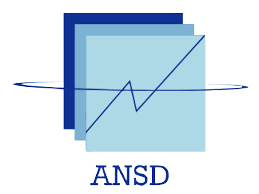
\includegraphics[width=4cm]{Logo3.png} \\[0.1cm]  
        
        \textbf{\large École Nationale de la Statistique et de l'Analyse Économique Pierre Ndiaye (ENSAE)}\\[0.4cm]
        
\includegraphics[width=3cm]{Logo4.png} \\[0.1cm]
        
        \textbf{\LARGE PROJET STATISTIQUES SOUS R }\\[0.3cm]
        \textbf{\Huge \color{black} \textsf{TP9 : Merge des bases de données EHCVM 2018 et 2021}}\\[0.2cm]
        \rule{\linewidth}{0.2mm} \\[0.5cm]
        
        \begin{minipage}{0.5\textwidth}
    \begin{flushleft} \large
        \emph{\textsf{Rédigé par :}}\\
        \textbf{Mame Balla BOUSSO}\\
        \textbf{Ameth FAYE}\\
        \textbf{EDIMA Biyenda Hildégarde}\\
        \textbf{Papa Amadou NIANG}\\
        \textit{Elèves ingénieurs statisticiens économistes}
    \end{flushleft}
\end{minipage}
        \hfill
        \begin{minipage}{0.4\textwidth}
            \begin{flushright} \large
                \emph{\textsf{Sous la supervision de :}} \\
                \textbf{M. Aboubacar HEMA}\\
                \textit{ANALYSTE DE RECHERCHE CHEZ IFPRI }
            \end{flushright}
        \end{minipage}

        \vfill

        {\large \textsf{Année scolaire : 2024/2025}}\\[0.5cm]
        
    \end{center}
\end{titlepage}

\hypertarget{introduction}{%
\section{Introduction}\label{introduction}}

Dans le cadre de ce projet, nous combinons les observations de la base
de données EHCVM 2021 avec celles de 2018 via une opération d'append.
L'objectif principal est d'harmoniser les variables afin d'assurer la
cohérence de l'ensemble des données pour des analyses ultérieures.

Pour ce faire, nous suivrons les étapes suivantes :

\begin{enumerate}
\def\labelenumi{\arabic{enumi}.}
\tightlist
\item
  \textbf{Extraction et listing des variables labelisées (Base 2018)}

  \begin{itemize}
  \tightlist
  \item
    Extraire et vérifier la liste des variables labelisées dans la base
    2018;\\
  \item
    Documenter les codes et modalités associées à chaque variable.
  \end{itemize}
\item
  \textbf{Extraction et listing des variables correspondantes (Base
  2021)}

  \begin{itemize}
  \tightlist
  \item
    Réaliser la même extraction pour la base 2021.\\
  \item
    Identifier les différences éventuelles dans les codes ou modalités
    par rapport à 2018.
  \end{itemize}
\item
  \textbf{Analyse comparative et plan d'harmonisation}

  \begin{itemize}
  \tightlist
  \item
    Comparer les listes de variables des deux bases.\\
  \item
    Identifier les écarts et proposer des solutions (recodage, ajout de
    modalités, renommage avec suffixe, etc.) pour harmoniser les
    variables fixes.\\
  \item
    Documenter le plan d'action détaillé.
  \end{itemize}
\item
  \textbf{Mise en œuvre et contrôle qualité}

  \begin{itemize}
  \tightlist
  \item
    Appliquer le plan d'harmonisation sur les données.\\
  \item
    Effectuer l'append des observations de 2021 à la base 2018.\\
  \item
    Réaliser des tests pour vérifier la cohérence globale des données.
  \end{itemize}
\end{enumerate}

Les sections suivantes du document illustrent la démarche avec le
chargement et la description des bases, l'identification des variables
communes et distinctes (avec ajout de suffixes pour distinguer
d'éventuelles différences de codification), le recodage des variables
nécessitant un ajustement, puis la combinaison finale des bases.

\hypertarget{chargement-des-donnuxe9es-et-description}{%
\section{Chargement des Données et
Description}\label{chargement-des-donnuxe9es-et-description}}

\begin{Shaded}
\begin{Highlighting}[]
\CommentTok{\# Chargement des bases de données}
\NormalTok{base2018 }\OtherTok{\textless{}{-}}\NormalTok{ haven}\SpecialCharTok{::}\FunctionTok{read\_dta}\NormalTok{(}\StringTok{"data/ehcvm\_welfare\_SEN2018.dta"}\NormalTok{)}
\NormalTok{base2021 }\OtherTok{\textless{}{-}}\NormalTok{ haven}\SpecialCharTok{::}\FunctionTok{read\_dta}\NormalTok{(}\StringTok{"data/ehcvm\_welfare\_sen2021.dta"}\NormalTok{)}

\CommentTok{\# Affichage du nombre d\textquotesingle{}observations et de variables pour chaque base}
\FunctionTok{cat}\NormalTok{(}\StringTok{"Dimensions de la base 2018 :"}\NormalTok{, }\FunctionTok{dim}\NormalTok{(base2018), }\StringTok{"}\SpecialCharTok{\textbackslash{}n}\StringTok{"}\NormalTok{)}
\end{Highlighting}
\end{Shaded}

\begin{verbatim}
## Dimensions de la base 2018 : 7156 35
\end{verbatim}

\begin{Shaded}
\begin{Highlighting}[]
\FunctionTok{cat}\NormalTok{(}\StringTok{"Dimensions de la base 2021 :"}\NormalTok{, }\FunctionTok{dim}\NormalTok{(base2021), }\StringTok{"}\SpecialCharTok{\textbackslash{}n}\StringTok{"}\NormalTok{)}
\end{Highlighting}
\end{Shaded}

\begin{verbatim}
## Dimensions de la base 2021 : 7120 47
\end{verbatim}

\begin{Shaded}
\begin{Highlighting}[]
\CommentTok{\# Aperçu rapide des données}
\FunctionTok{summary}\NormalTok{(base2018)}
\end{Highlighting}
\end{Shaded}

\begin{verbatim}
##    country               year           hhid            grappe     
##  Length:7156        Min.   :2018   Min.   :  1001   Min.   :  1.0  
##  Class :character   1st Qu.:2018   1st Qu.:151002   1st Qu.:151.0  
##  Mode  :character   Median :2018   Median :300003   Median :300.0  
##                     Mean   :2018   Mean   :299934   Mean   :299.9  
##                     3rd Qu.:2018   3rd Qu.:449010   3rd Qu.:449.0  
##                     Max.   :2018   Max.   :598012   Max.   :598.0  
##                                                                    
##      menage           vague            zae            region      
##  Min.   : 1.000   Min.   :1.000   Min.   :1.000   Min.   : 1.000  
##  1st Qu.: 3.000   1st Qu.:1.000   1st Qu.:2.000   1st Qu.: 3.000  
##  Median : 6.000   Median :2.000   Median :4.000   Median : 7.000  
##  Mean   : 6.491   Mean   :1.501   Mean   :3.466   Mean   : 6.781  
##  3rd Qu.: 9.000   3rd Qu.:2.000   3rd Qu.:5.000   3rd Qu.:10.000  
##  Max.   :12.000   Max.   :2.000   Max.   :6.000   Max.   :14.000  
##                                                                   
##      milieu         hhweight           hhsize          eqadu1      
##  Min.   :1.000   Min.   :  15.29   Min.   : 1.00   Min.   : 0.660  
##  1st Qu.:1.000   1st Qu.: 120.57   1st Qu.: 5.00   1st Qu.: 3.960  
##  Median :1.000   Median : 203.88   Median : 8.00   Median : 5.982  
##  Mean   :1.449   Mean   : 250.38   Mean   : 9.24   Mean   : 6.867  
##  3rd Qu.:2.000   3rd Qu.: 322.74   3rd Qu.:12.00   3rd Qu.: 8.720  
##  Max.   :2.000   Max.   :2808.65   Max.   :56.00   Max.   :41.240  
##                                                                    
##      eqadu2          hgender           hage           hmstat     
##  Min.   : 1.000   Min.   :1.000   Min.   :17.00   Min.   :1.000  
##  1st Qu.: 3.167   1st Qu.:1.000   1st Qu.:41.00   1st Qu.:2.000  
##  Median : 4.333   Median :1.000   Median :51.00   Median :2.000  
##  Mean   : 4.811   Mean   :1.262   Mean   :51.49   Mean   :2.704  
##  3rd Qu.: 5.984   3rd Qu.:2.000   3rd Qu.:62.00   3rd Qu.:3.000  
##  Max.   :23.706   Max.   :2.000   Max.   :99.00   Max.   :7.000  
##                                                   NA's   :2      
##    hreligion        hnation           halfab           heduc      
##  Min.   :1.000   Min.   : 2.000   Min.   :0.0000   Min.   :1.000  
##  1st Qu.:1.000   1st Qu.: 7.000   1st Qu.:0.0000   1st Qu.:1.000  
##  Median :1.000   Median : 7.000   Median :0.0000   Median :1.000  
##  Mean   :1.061   Mean   : 7.024   Mean   :0.4707   Mean   :2.188  
##  3rd Qu.:1.000   3rd Qu.: 7.000   3rd Qu.:1.0000   3rd Qu.:3.000  
##  Max.   :5.000   Max.   :12.000   Max.   :1.0000   Max.   :9.000  
##                                                                   
##     hdiploma          hhandig           hactiv7j       hactiv12m   
##  Min.   : 0.0000   Min.   :0.00000   Min.   :1.000   Min.   :1.00  
##  1st Qu.: 0.0000   1st Qu.:0.00000   1st Qu.:1.000   1st Qu.:1.00  
##  Median : 0.0000   Median :0.00000   Median :1.000   Median :1.00  
##  Mean   : 0.6385   Mean   :0.09083   Mean   :1.975   Mean   :1.49  
##  3rd Qu.: 0.0000   3rd Qu.:0.00000   3rd Qu.:2.000   3rd Qu.:1.00  
##  Max.   :10.0000   Max.   :1.00000   Max.   :5.000   Max.   :3.00  
##                                                                    
##     hbranch          hsectins          hcsp             dali         
##  Min.   : 1.000   Min.   :1.000   Min.   : 1.000   Min.   :  113187  
##  1st Qu.: 1.000   1st Qu.:3.000   1st Qu.: 5.000   1st Qu.: 1143473  
##  Median : 6.000   Median :3.000   Median : 9.000   Median : 1746986  
##  Mean   : 5.324   Mean   :2.894   Mean   : 7.428   Mean   : 2063862  
##  3rd Qu.: 9.000   3rd Qu.:3.000   3rd Qu.: 9.000   3rd Qu.: 2575472  
##  Max.   :11.000   Max.   :6.000   Max.   :10.000   Max.   :31295272  
##  NA's   :1722     NA's   :1722    NA's   :1722                       
##       dnal                dtot               pcexp               zzae       
##  Min.   :    27585   Min.   :   278116   Min.   :   64161   Min.   :296311  
##  1st Qu.:   990977   1st Qu.:  2268859   1st Qu.:  300149   1st Qu.:305745  
##  Median :  1632298   Median :  3484846   Median :  442539   Median :326047  
##  Mean   :  2268143   Mean   :  4332005   Mean   :  615630   Mean   :332244  
##  3rd Qu.:  2771981   3rd Qu.:  5391925   3rd Qu.:  697134   3rd Qu.:348125  
##  Max.   :221582921   Max.   :227607152   Max.   :14286279   Max.   :391340  
##                                                                             
##       zref           def_spa          def_temp     
##  Min.   :333441   Min.   :0.8886   Min.   :0.9916  
##  1st Qu.:333441   1st Qu.:0.9169   1st Qu.:0.9916  
##  Median :333441   Median :0.9778   Median :0.9955  
##  Mean   :333441   Mean   :0.9964   Mean   :1.0015  
##  3rd Qu.:333441   3rd Qu.:1.0440   3rd Qu.:1.0089  
##  Max.   :333441   Max.   :1.1736   Max.   :1.0147  
## 
\end{verbatim}

\begin{Shaded}
\begin{Highlighting}[]
\FunctionTok{summary}\NormalTok{(base2021)}
\end{Highlighting}
\end{Shaded}

\begin{verbatim}
##      grappe          menage         country               year     
##  Min.   :  2.0   Min.   : 1.000   Length:7120        Min.   :2021  
##  1st Qu.:152.0   1st Qu.: 4.000   Class :character   1st Qu.:2021  
##  Median :301.0   Median : 7.000   Mode  :character   Median :2021  
##  Mean   :300.7   Mean   : 7.187                      Mean   :2021  
##  3rd Qu.:450.0   3rd Qu.:10.000                      3rd Qu.:2021  
##  Max.   :598.0   Max.   :19.000                      Max.   :2021  
##                                                                    
##       hhid           vague           month                 zae        
##  Min.   :  201   Min.   :1.000   Min.   :2021-11-01   Min.   : 1.000  
##  1st Qu.:15208   1st Qu.:1.000   1st Qu.:2021-12-01   1st Qu.: 5.000  
##  Median :30103   Median :2.000   Median :2022-04-01   Median : 7.000  
##  Mean   :30082   Mean   :1.503   Mean   :2022-02-16   Mean   : 6.712  
##  3rd Qu.:45004   3rd Qu.:2.000   3rd Qu.:2022-05-01   3rd Qu.: 9.000  
##  Max.   :59812   Max.   :2.000   Max.   :2022-07-01   Max.   :11.000  
##                                                                       
##      region           milieu         hhweight           hhsize      
##  Min.   : 1.000   Min.   :1.000   Min.   :  17.73   Min.   : 1.000  
##  1st Qu.: 3.000   1st Qu.:1.000   1st Qu.: 131.07   1st Qu.: 5.000  
##  Median : 7.000   Median :1.000   Median : 221.81   Median : 8.000  
##  Mean   : 6.799   Mean   :1.449   Mean   : 297.44   Mean   : 8.747  
##  3rd Qu.:10.000   3rd Qu.:2.000   3rd Qu.: 380.29   3rd Qu.:11.000  
##  Max.   :14.000   Max.   :2.000   Max.   :3081.51   Max.   :53.000  
##                                                                     
##      eqadu1           eqadu2          hgender           hage       
##  Min.   : 0.660   Min.   : 1.000   Min.   :1.000   Min.   : 16.00  
##  1st Qu.: 3.940   1st Qu.: 3.008   1st Qu.:1.000   1st Qu.: 44.00  
##  Median : 5.790   Median : 4.180   Median :1.000   Median : 54.00  
##  Mean   : 6.589   Mean   : 4.625   Mean   :1.284   Mean   : 54.08  
##  3rd Qu.: 8.350   3rd Qu.: 5.762   3rd Qu.:2.000   3rd Qu.: 64.00  
##  Max.   :40.265   Max.   :22.882   Max.   :2.000   Max.   :101.00  
##                                                                    
##      hmstat        hreligion        hnation         hethnie      
##  Min.   :1.000   Min.   :1.000   Min.   : 4.00   Min.   : 1.000  
##  1st Qu.:2.000   1st Qu.:1.000   1st Qu.:13.00   1st Qu.: 1.000  
##  Median :2.000   Median :1.000   Median :13.00   Median : 3.000  
##  Mean   :2.805   Mean   :1.058   Mean   :12.95   Mean   : 3.096  
##  3rd Qu.:3.000   3rd Qu.:1.000   3rd Qu.:13.00   3rd Qu.: 3.000  
##  Max.   :7.000   Max.   :5.000   Max.   :18.00   Max.   :13.000  
##                                                  NA's   :82      
##      halfa            halfa2           heduc          hdiploma      
##  Min.   :0.0000   Min.   :0.0000   Min.   :1.000   Min.   : 0.0000  
##  1st Qu.:0.0000   1st Qu.:0.0000   1st Qu.:1.000   1st Qu.: 0.0000  
##  Median :1.0000   Median :0.0000   Median :1.000   Median : 0.0000  
##  Mean   :0.5117   Mean   :0.4947   Mean   :2.112   Mean   : 0.5622  
##  3rd Qu.:1.0000   3rd Qu.:1.0000   3rd Qu.:3.000   3rd Qu.: 0.0000  
##  Max.   :1.0000   Max.   :1.0000   Max.   :9.000   Max.   :10.0000  
##                                                                     
##     hhandig           hactiv7j       hactiv12m        hbranch      
##  Min.   :0.00000   Min.   :1.000   Min.   :1.000   Min.   :  1.00  
##  1st Qu.:0.00000   1st Qu.:1.000   1st Qu.:1.000   1st Qu.:  1.00  
##  Median :0.00000   Median :1.000   Median :1.000   Median :  5.00  
##  Mean   :0.08919   Mean   :2.067   Mean   :1.382   Mean   :  6.36  
##  3rd Qu.:0.00000   3rd Qu.:5.000   3rd Qu.:1.000   3rd Qu.:  8.00  
##  Max.   :1.00000   Max.   :5.000   Max.   :3.000   Max.   :930.00  
##                                                    NA's   :1838    
##     hsectins          hcsp             dali               dnal         
##  Min.   :1.000   Min.   : 1.000   Min.   :   64205   Min.   :  129749  
##  1st Qu.:3.000   1st Qu.: 9.000   1st Qu.: 1325492   1st Qu.:  972937  
##  Median :3.000   Median : 9.000   Median : 1956762   Median : 1595027  
##  Mean   :2.937   Mean   : 7.717   Mean   : 2276262   Mean   : 2029004  
##  3rd Qu.:3.000   3rd Qu.: 9.000   3rd Qu.: 2840293   3rd Qu.: 2556010  
##  Max.   :6.000   Max.   :10.000   Max.   :15144512   Max.   :19917053  
##  NA's   :1359    NA's   :1326                                          
##       dtot              pcexp              zzae             zref       
##  Min.   :  235210   Min.   :  57610   Min.   :331925   Min.   :369666  
##  1st Qu.: 2432066   1st Qu.: 328408   1st Qu.:335734   1st Qu.:369666  
##  Median : 3614746   Median : 472561   Median :373110   Median :369666  
##  Mean   : 4305266   Mean   : 621198   Mean   :371487   Mean   :369666  
##  3rd Qu.: 5359042   3rd Qu.: 724571   3rd Qu.:385554   3rd Qu.:369666  
##  Max.   :29248050   Max.   :9990532   Max.   :424179   Max.   :369666  
##                                                                        
##     def_spa          def_temp      def_temp_prix2021m11  def_temp_cpi   
##  Min.   :0.8979   Min.   :0.9455   Min.   :1.000        Min.   :0.9743  
##  1st Qu.:0.9082   1st Qu.:0.9833   1st Qu.:1.001        1st Qu.:0.9752  
##  Median :1.0093   Median :0.9949   Median :1.020        Median :0.9935  
##  Mean   :1.0049   Mean   :0.9981   Mean   :1.020        Mean   :0.9935  
##  3rd Qu.:1.0430   3rd Qu.:1.0200   3rd Qu.:1.027        3rd Qu.:1.0009  
##  Max.   :1.1475   Max.   :1.0590   Max.   :1.087        Max.   :1.0587  
##                                                                         
##   def_temp_adj        zali0             dtet           monthly_cpi   
##  Min.   :0.9606   Min.   :196233   Min.   :   50712   Min.   :117.2  
##  1st Qu.:0.9991   1st Qu.:196233   1st Qu.:  317994   1st Qu.:117.4  
##  Median :1.0109   Median :196233   Median :  469028   Median :119.6  
##  Mean   :1.0140   Mean   :196233   Mean   :  641538   Mean   :119.6  
##  3rd Qu.:1.0363   3rd Qu.:196233   3rd Qu.:  746041   3rd Qu.:120.4  
##  Max.   :1.0760   Max.   :196233   Max.   :10366096   Max.   :127.4  
##                                                                      
##     cpi2017         icp2017         dollars        
##  Min.   :1.097   Min.   :238.6   Min.   :  0.5376  
##  1st Qu.:1.097   1st Qu.:238.6   1st Qu.:  3.2473  
##  Median :1.097   Median :238.6   Median :  4.7915  
##  Mean   :1.097   Mean   :238.6   Mean   :  6.5526  
##  3rd Qu.:1.097   3rd Qu.:238.6   3rd Qu.:  7.6134  
##  Max.   :1.097   Max.   :238.6   Max.   :102.5809  
## 
\end{verbatim}

\hypertarget{identification-des-variables-communes-et-diffuxe9rentes}{%
\section{Identification des variables communes et
différentes}\label{identification-des-variables-communes-et-diffuxe9rentes}}

Dans cette section, nous identifions les variables présentes dans les
deux bases et celles qui diffèrent. Pour les variables communes, nous
vérifierons que leur codification est identique. Pour les variables
présentant des différences, nous ajouterons le suffixe \texttt{\_2018}
ou \texttt{\_2021} afin de bien distinguer l'origine de chaque modalité.

\begin{Shaded}
\begin{Highlighting}[]
\CommentTok{\# Récupération des noms de colonnes}
\NormalTok{vars\_2018 }\OtherTok{\textless{}{-}} \FunctionTok{names}\NormalTok{(base2018)}
\NormalTok{vars\_2021 }\OtherTok{\textless{}{-}} \FunctionTok{names}\NormalTok{(base2021)}

\CommentTok{\# Variables communes aux deux bases}
\NormalTok{vars\_communes }\OtherTok{\textless{}{-}} \FunctionTok{intersect}\NormalTok{(vars\_2018, vars\_2021)}
\FunctionTok{cat}\NormalTok{(}\StringTok{"Variables communes :"}\NormalTok{, vars\_communes, }\StringTok{"}\SpecialCharTok{\textbackslash{}n}\StringTok{"}\NormalTok{)}
\end{Highlighting}
\end{Shaded}

\begin{verbatim}
## Variables communes : country year hhid grappe menage vague zae region milieu hhweight hhsize eqadu1 eqadu2 hgender hage hmstat hreligion hnation heduc hdiploma hhandig hactiv7j hactiv12m hbranch hsectins hcsp dali dnal dtot pcexp zzae zref def_spa def_temp
\end{verbatim}

\begin{Shaded}
\begin{Highlighting}[]
\CommentTok{\# Variables spécifiques à chaque base}
\NormalTok{vars\_uniques\_2018 }\OtherTok{\textless{}{-}} \FunctionTok{setdiff}\NormalTok{(vars\_2018, vars\_2021)}
\NormalTok{vars\_uniques\_2021 }\OtherTok{\textless{}{-}} \FunctionTok{setdiff}\NormalTok{(vars\_2021, vars\_2018)}
\FunctionTok{cat}\NormalTok{(}\StringTok{"Variables spécifiques à 2018 :"}\NormalTok{, vars\_uniques\_2018, }\StringTok{"}\SpecialCharTok{\textbackslash{}n}\StringTok{"}\NormalTok{)}
\end{Highlighting}
\end{Shaded}

\begin{verbatim}
## Variables spécifiques à 2018 : halfab
\end{verbatim}

\begin{Shaded}
\begin{Highlighting}[]
\FunctionTok{cat}\NormalTok{(}\StringTok{"Variables spécifiques à 2021 :"}\NormalTok{, vars\_uniques\_2021, }\StringTok{"}\SpecialCharTok{\textbackslash{}n}\StringTok{"}\NormalTok{)}
\end{Highlighting}
\end{Shaded}

\begin{verbatim}
## Variables spécifiques à 2021 : month hethnie halfa halfa2 def_temp_prix2021m11 def_temp_cpi def_temp_adj zali0 dtet monthly_cpi cpi2017 icp2017 dollars
\end{verbatim}

\begin{itemize}
\item
  \textbf{Les variables communes} :\\
  Une intersection des noms de colonnes révèle 34 variables partagées
  entre les deux bases (par exemple, \emph{country}, \emph{year},
  \emph{hhid}, etc.). Pour ces variables, il sera possible de vérifier
  directement que leur codification est identique.
\item
  \textbf{Les variables spécifiques à chaque base} :\\
  La base 2018 présente une variable unique (\emph{halphab}), tandis que
  la base 2021 (affichée ici comme 2021) contient 12 variables
  spécifiques (parmi lesquelles \emph{month}, \emph{hethnie},
  \emph{halfa}, \emph{halfa2}, etc.).\\
  Il est important de noter que la variable \emph{halphab} de 2018 a
  pour correspondant \emph{halpha2} dans la base 2021. Cela indique
  qu'une harmonisation manuelle est nécessaire pour aligner ces deux
  variables équivalentes avant de procéder à la fusion des données.
\end{itemize}

\hypertarget{recodage-et-harmonisation}{%
\section{Recodage et harmonisation}\label{recodage-et-harmonisation}}

Nous passons maintenant à l'analyse des variables communes pour vérifier
leur codification. Pour les variables dont les modalités diffèrent entre
2018 et 2021, nous appliquons un recodage et/ou ajoutons un suffixe afin
de conserver la provenance des données.

Dans un premier temps, nous allons faire correspondre la variable halfa2
à la variable halphab en le renommant :

\begin{Shaded}
\begin{Highlighting}[]
\FunctionTok{library}\NormalTok{(dplyr)}

\NormalTok{base2021 }\OtherTok{\textless{}{-}}\NormalTok{ base2021 }\SpecialCharTok{\%\textgreater{}\%} 
  \FunctionTok{rename}\NormalTok{(}\AttributeTok{halfab =}\NormalTok{ halfa2)}
\end{Highlighting}
\end{Shaded}

Nous allons ensuite vérifier si les variables communes sont codifiés de
la même manière :

\begin{Shaded}
\begin{Highlighting}[]
\CommentTok{\# Charger les bibliothèques nécessaires}
\FunctionTok{library}\NormalTok{(dplyr)}
\FunctionTok{library}\NormalTok{(labelled)}
\FunctionTok{library}\NormalTok{(knitr)}
\FunctionTok{library}\NormalTok{(kableExtra)}

\CommentTok{\# Liste des variables à convertir en facteur}
\NormalTok{vars }\OtherTok{\textless{}{-}} \FunctionTok{c}\NormalTok{(}\StringTok{"zae"}\NormalTok{, }\StringTok{"region"}\NormalTok{, }\StringTok{"milieu"}\NormalTok{, }\StringTok{"hgender"}\NormalTok{, }\StringTok{"hmstat"}\NormalTok{, }\StringTok{"hreligion"}\NormalTok{, }\StringTok{"hnation"}\NormalTok{,}
          \StringTok{"halfab"}\NormalTok{, }\StringTok{"heduc"}\NormalTok{, }\StringTok{"hdiploma"}\NormalTok{, }\StringTok{"hhandig"}\NormalTok{, }\StringTok{"hactiv7j"}\NormalTok{, }\StringTok{"hactiv12m"}\NormalTok{, }
          \StringTok{"hbranch"}\NormalTok{, }\StringTok{"hsectins"}\NormalTok{, }\StringTok{"hcsp"}\NormalTok{)}


\CommentTok{\# Fonction pour extraire les codes et libellés d\textquotesingle{}une variable}
\NormalTok{extract\_labels }\OtherTok{\textless{}{-}} \ControlFlowTok{function}\NormalTok{(var) \{}
  \ControlFlowTok{if}\NormalTok{ (}\SpecialCharTok{!}\FunctionTok{is.null}\NormalTok{(}\FunctionTok{attr}\NormalTok{(base2018[[var]], }\StringTok{"labels"}\NormalTok{))) \{  }\CommentTok{\# Vérifie si la variable a des labels}
\NormalTok{    N }\OtherTok{\textless{}{-}} \FunctionTok{names}\NormalTok{(}\FunctionTok{attr}\NormalTok{(base2018[[var]], }\StringTok{"labels"}\NormalTok{))  }\CommentTok{\# Libellés}
\NormalTok{    L }\OtherTok{\textless{}{-}} \FunctionTok{unname}\NormalTok{(}\FunctionTok{attr}\NormalTok{(base2018[[var]], }\StringTok{"labels"}\NormalTok{)) }\CommentTok{\# Codes}
\NormalTok{    df }\OtherTok{\textless{}{-}} \FunctionTok{data.frame}\NormalTok{(}\AttributeTok{Variable =}\NormalTok{ var, }\AttributeTok{Code =}\NormalTok{ L, Libellé }\OtherTok{=}\NormalTok{ N)}
    \FunctionTok{return}\NormalTok{(df)}
\NormalTok{  \} }\ControlFlowTok{else}\NormalTok{ \{}
    \FunctionTok{return}\NormalTok{(}\ConstantTok{NULL}\NormalTok{) }\CommentTok{\# Retourne NULL si pas de labels}
\NormalTok{  \}}
\NormalTok{\}}

\CommentTok{\# Appliquer la fonction à toutes les variables}
\NormalTok{labels\_list }\OtherTok{\textless{}{-}} \FunctionTok{lapply}\NormalTok{(vars, extract\_labels)}

\CommentTok{\# Supprimer les NULL et fusionner les résultats en un seul tableau}
\NormalTok{labels\_table }\OtherTok{\textless{}{-}} \FunctionTok{bind\_rows}\NormalTok{(labels\_list)}

\CommentTok{\# Afficher sous forme de tableau}
\FunctionTok{kable}\NormalTok{(labels\_table, }\AttributeTok{caption =} \StringTok{"Codes et libellés des variables"}\NormalTok{)}
\end{Highlighting}
\end{Shaded}

\begin{longtable}[]{@{}
  >{\raggedright\arraybackslash}p{(\columnwidth - 4\tabcolsep) * \real{0.1333}}
  >{\raggedleft\arraybackslash}p{(\columnwidth - 4\tabcolsep) * \real{0.0667}}
  >{\raggedright\arraybackslash}p{(\columnwidth - 4\tabcolsep) * \real{0.8000}}@{}}
\caption{Codes et libellés des variables}\tabularnewline
\toprule\noalign{}
\begin{minipage}[b]{\linewidth}\raggedright
Variable
\end{minipage} & \begin{minipage}[b]{\linewidth}\raggedleft
Code
\end{minipage} & \begin{minipage}[b]{\linewidth}\raggedright
Libellé
\end{minipage} \\
\midrule\noalign{}
\endfirsthead
\toprule\noalign{}
\begin{minipage}[b]{\linewidth}\raggedright
Variable
\end{minipage} & \begin{minipage}[b]{\linewidth}\raggedleft
Code
\end{minipage} & \begin{minipage}[b]{\linewidth}\raggedright
Libellé
\end{minipage} \\
\midrule\noalign{}
\endhead
\bottomrule\noalign{}
\endlastfoot
region & 1 & DAKAR \\
region & 2 & ZIGUINCHOR \\
region & 3 & DIOURBEL \\
region & 4 & SAINT-LOUIS \\
region & 5 & TAMBACOUNDA \\
region & 6 & KAOLACK \\
region & 7 & THIES \\
region & 8 & LOUGA \\
region & 9 & FATICK \\
region & 10 & KOLDA \\
region & 11 & MATAM \\
region & 12 & KAFFRINE \\
region & 13 & KEDOUGOU \\
region & 14 & SEDHIOU \\
milieu & 1 & Urbain \\
milieu & 2 & Rural \\
hgender & 1 & Masculin \\
hgender & 2 & Féminin \\
hmstat & 1 & Célibataire \\
hmstat & 2 & Marié(e) monogame \\
hmstat & 3 & Marié(e) polygame \\
hmstat & 4 & Union libre \\
hmstat & 5 & Veuf(ve) \\
hmstat & 6 & Divorcé(e) \\
hmstat & 7 & Séparé(e) \\
hreligion & 1 & Musulman \\
hreligion & 2 & Chrétien \\
hreligion & 3 & Animiste \\
hreligion & 4 & Autre Réligion \\
hreligion & 5 & Sans Réligion \\
hnation & 1 & Benin \\
hnation & 2 & Burkina Faso \\
hnation & 3 & Côte d'Ivoire \\
hnation & 4 & Guinée Bissau \\
hnation & 5 & Mali \\
hnation & 6 & Niger \\
hnation & 7 & Sénégal \\
hnation & 8 & Togo \\
hnation & 9 & Nigéria \\
hnation & 10 & Autre CEDEAO \\
hnation & 11 & Autre Afrique \\
hnation & 12 & Autre pays hors Afrique \\
halfab & 0 & Non \\
halfab & 1 & Oui \\
heduc & 1 & Aucun \\
heduc & 2 & Maternelle \\
heduc & 3 & Primaire \\
heduc & 4 & Second. gl 1 \\
heduc & 5 & Second. tech. 1 \\
heduc & 6 & Second. gl 2 \\
heduc & 7 & Second. tech. 2 \\
heduc & 8 & Postsecondaire \\
heduc & 9 & Superieur \\
hdiploma & 0 & Aucun \\
hdiploma & 1 & CEP/CFEE \\
hdiploma & 2 & BEPC/BFEM \\
hdiploma & 3 & CAP \\
hdiploma & 4 & BT \\
hdiploma & 5 & BAC \\
hdiploma & 6 & DEUG, DUT, BTS \\
hdiploma & 7 & Licence \\
hdiploma & 8 & Maitrise \\
hdiploma & 9 & Master/DEA/DESS \\
hdiploma & 10 & Doctorat/Phd \\
hhandig & 0 & Non \\
hhandig & 1 & Oui \\
hactiv7j & 1 & Occupe \\
hactiv7j & 2 & Chomeur \\
hactiv7j & 3 & TF cherchant emploi \\
hactiv7j & 4 & TF cherchant pas \\
hactiv7j & 5 & Inactif \\
hactiv7j & 6 & Moins de 5 ans \\
hactiv12m & 1 & Occupe \\
hactiv12m & 2 & Trav. fam. \\
hactiv12m & 3 & Non occupe \\
hactiv12m & 4 & Moins de 5 ans \\
hbranch & 1 & Agriculture \\
hbranch & 2 & Elevage/peche \\
hbranch & 3 & Indust. extr. \\
hbranch & 4 & Autr. indust. \\
hbranch & 5 & BTP \\
hbranch & 6 & Commerce \\
hbranch & 7 & Restaurant/Hotel \\
hbranch & 8 & Trans./Comm. \\
hbranch & 9 & Education/Sante \\
hbranch & 10 & Services perso. \\
hbranch & 11 & Aut. services \\
hsectins & 1 & Etat/Collectivités locales \\
hsectins & 2 & Entreprise publique/ parapublique \\
hsectins & 3 & Entreprise Privée \\
hsectins & 4 & Entreprise associative \\
hsectins & 5 & Ménage comme employeur de personnel domestique \\
hsectins & 6 & Organisme international /Ambassade \\
hcsp & 1 & Cadre supérieur \\
hcsp & 2 & Cadre moyen/agent de maîtrise \\
hcsp & 3 & Ouvrier ou employé qualifié \\
hcsp & 4 & Ouvrier ou employé non qualifié \\
hcsp & 5 & Manœuvre, aide ménagère \\
hcsp & 6 & Stagiaire ou Apprenti rénuméré \\
hcsp & 7 & Stagiaire ou Apprenti non rénuméré \\
hcsp & 8 & Travailleur familial contribuant à une entreprise
familiale \\
hcsp & 9 & Travailleur pour compte propre \\
hcsp & 10 & Patron \\
\end{longtable}

\begin{Shaded}
\begin{Highlighting}[]
\FunctionTok{kable}\NormalTok{(labels\_table, }\AttributeTok{caption =} \StringTok{"Codes et libellés des variables"}\NormalTok{) }\SpecialCharTok{\%\textgreater{}\%}
  \FunctionTok{kable\_styling}\NormalTok{(}\AttributeTok{bootstrap\_options =} \FunctionTok{c}\NormalTok{(}\StringTok{"striped"}\NormalTok{, }\StringTok{"hover"}\NormalTok{, }\StringTok{"condensed"}\NormalTok{, }\StringTok{"responsive"}\NormalTok{), }
                \AttributeTok{full\_width =} \ConstantTok{FALSE}\NormalTok{, }\AttributeTok{position =} \StringTok{"center"}\NormalTok{) }\SpecialCharTok{\%\textgreater{}\%}
  \FunctionTok{column\_spec}\NormalTok{(}\DecValTok{1}\NormalTok{, }\AttributeTok{bold =} \ConstantTok{TRUE}\NormalTok{, }\AttributeTok{color =} \StringTok{"blue"}\NormalTok{) }\SpecialCharTok{\%\textgreater{}\%}
  \FunctionTok{column\_spec}\NormalTok{(}\DecValTok{2}\NormalTok{, }\AttributeTok{bold =} \ConstantTok{TRUE}\NormalTok{) }\SpecialCharTok{\%\textgreater{}\%}
  \FunctionTok{column\_spec}\NormalTok{(}\DecValTok{3}\NormalTok{, }\AttributeTok{width =} \StringTok{"8cm"}\NormalTok{)}
\end{Highlighting}
\end{Shaded}

\begin{longtable}[t]{>{}l>{}r>{\raggedright\arraybackslash}p{8cm}}
\caption{\label{tab:recodage-harmonisation-2}Codes et libellés des variables}\\
\toprule
Variable & Code & Libellé\\
\midrule
\textcolor{blue}{\textbf{region}} & \textbf{1} & DAKAR\\
\textcolor{blue}{\textbf{region}} & \textbf{2} & ZIGUINCHOR\\
\textcolor{blue}{\textbf{region}} & \textbf{3} & DIOURBEL\\
\textcolor{blue}{\textbf{region}} & \textbf{4} & SAINT-LOUIS\\
\textcolor{blue}{\textbf{region}} & \textbf{5} & TAMBACOUNDA\\
\addlinespace
\textcolor{blue}{\textbf{region}} & \textbf{6} & KAOLACK\\
\textcolor{blue}{\textbf{region}} & \textbf{7} & THIES\\
\textcolor{blue}{\textbf{region}} & \textbf{8} & LOUGA\\
\textcolor{blue}{\textbf{region}} & \textbf{9} & FATICK\\
\textcolor{blue}{\textbf{region}} & \textbf{10} & KOLDA\\
\addlinespace
\textcolor{blue}{\textbf{region}} & \textbf{11} & MATAM\\
\textcolor{blue}{\textbf{region}} & \textbf{12} & KAFFRINE\\
\textcolor{blue}{\textbf{region}} & \textbf{13} & KEDOUGOU\\
\textcolor{blue}{\textbf{region}} & \textbf{14} & SEDHIOU\\
\textcolor{blue}{\textbf{milieu}} & \textbf{1} & Urbain\\
\addlinespace
\textcolor{blue}{\textbf{milieu}} & \textbf{2} & Rural\\
\textcolor{blue}{\textbf{hgender}} & \textbf{1} & Masculin\\
\textcolor{blue}{\textbf{hgender}} & \textbf{2} & Féminin\\
\textcolor{blue}{\textbf{hmstat}} & \textbf{1} & Célibataire\\
\textcolor{blue}{\textbf{hmstat}} & \textbf{2} & Marié(e) monogame\\
\addlinespace
\textcolor{blue}{\textbf{hmstat}} & \textbf{3} & Marié(e) polygame\\
\textcolor{blue}{\textbf{hmstat}} & \textbf{4} & Union libre\\
\textcolor{blue}{\textbf{hmstat}} & \textbf{5} & Veuf(ve)\\
\textcolor{blue}{\textbf{hmstat}} & \textbf{6} & Divorcé(e)\\
\textcolor{blue}{\textbf{hmstat}} & \textbf{7} & Séparé(e)\\
\addlinespace
\textcolor{blue}{\textbf{hreligion}} & \textbf{1} & Musulman\\
\textcolor{blue}{\textbf{hreligion}} & \textbf{2} & Chrétien\\
\textcolor{blue}{\textbf{hreligion}} & \textbf{3} & Animiste\\
\textcolor{blue}{\textbf{hreligion}} & \textbf{4} & Autre Réligion\\
\textcolor{blue}{\textbf{hreligion}} & \textbf{5} & Sans Réligion\\
\addlinespace
\textcolor{blue}{\textbf{hnation}} & \textbf{1} & Benin\\
\textcolor{blue}{\textbf{hnation}} & \textbf{2} & Burkina Faso\\
\textcolor{blue}{\textbf{hnation}} & \textbf{3} & Côte d'Ivoire\\
\textcolor{blue}{\textbf{hnation}} & \textbf{4} & Guinée Bissau\\
\textcolor{blue}{\textbf{hnation}} & \textbf{5} & Mali\\
\addlinespace
\textcolor{blue}{\textbf{hnation}} & \textbf{6} & Niger\\
\textcolor{blue}{\textbf{hnation}} & \textbf{7} & Sénégal\\
\textcolor{blue}{\textbf{hnation}} & \textbf{8} & Togo\\
\textcolor{blue}{\textbf{hnation}} & \textbf{9} & Nigéria\\
\textcolor{blue}{\textbf{hnation}} & \textbf{10} & Autre CEDEAO\\
\addlinespace
\textcolor{blue}{\textbf{hnation}} & \textbf{11} & Autre Afrique\\
\textcolor{blue}{\textbf{hnation}} & \textbf{12} & Autre pays hors Afrique\\
\textcolor{blue}{\textbf{halfab}} & \textbf{0} & Non\\
\textcolor{blue}{\textbf{halfab}} & \textbf{1} & Oui\\
\textcolor{blue}{\textbf{heduc}} & \textbf{1} & Aucun\\
\addlinespace
\textcolor{blue}{\textbf{heduc}} & \textbf{2} & Maternelle\\
\textcolor{blue}{\textbf{heduc}} & \textbf{3} & Primaire\\
\textcolor{blue}{\textbf{heduc}} & \textbf{4} & Second. gl 1\\
\textcolor{blue}{\textbf{heduc}} & \textbf{5} & Second. tech. 1\\
\textcolor{blue}{\textbf{heduc}} & \textbf{6} & Second. gl 2\\
\addlinespace
\textcolor{blue}{\textbf{heduc}} & \textbf{7} & Second. tech. 2\\
\textcolor{blue}{\textbf{heduc}} & \textbf{8} & Postsecondaire\\
\textcolor{blue}{\textbf{heduc}} & \textbf{9} & Superieur\\
\textcolor{blue}{\textbf{hdiploma}} & \textbf{0} & Aucun\\
\textcolor{blue}{\textbf{hdiploma}} & \textbf{1} & CEP/CFEE\\
\addlinespace
\textcolor{blue}{\textbf{hdiploma}} & \textbf{2} & BEPC/BFEM\\
\textcolor{blue}{\textbf{hdiploma}} & \textbf{3} & CAP\\
\textcolor{blue}{\textbf{hdiploma}} & \textbf{4} & BT\\
\textcolor{blue}{\textbf{hdiploma}} & \textbf{5} & BAC\\
\textcolor{blue}{\textbf{hdiploma}} & \textbf{6} & DEUG, DUT, BTS\\
\addlinespace
\textcolor{blue}{\textbf{hdiploma}} & \textbf{7} & Licence\\
\textcolor{blue}{\textbf{hdiploma}} & \textbf{8} & Maitrise\\
\textcolor{blue}{\textbf{hdiploma}} & \textbf{9} & Master/DEA/DESS\\
\textcolor{blue}{\textbf{hdiploma}} & \textbf{10} & Doctorat/Phd\\
\textcolor{blue}{\textbf{hhandig}} & \textbf{0} & Non\\
\addlinespace
\textcolor{blue}{\textbf{hhandig}} & \textbf{1} & Oui\\
\textcolor{blue}{\textbf{hactiv7j}} & \textbf{1} & Occupe\\
\textcolor{blue}{\textbf{hactiv7j}} & \textbf{2} & Chomeur\\
\textcolor{blue}{\textbf{hactiv7j}} & \textbf{3} & TF cherchant emploi\\
\textcolor{blue}{\textbf{hactiv7j}} & \textbf{4} & TF cherchant pas\\
\addlinespace
\textcolor{blue}{\textbf{hactiv7j}} & \textbf{5} & Inactif\\
\textcolor{blue}{\textbf{hactiv7j}} & \textbf{6} & Moins de 5 ans\\
\textcolor{blue}{\textbf{hactiv12m}} & \textbf{1} & Occupe\\
\textcolor{blue}{\textbf{hactiv12m}} & \textbf{2} & Trav. fam.\\
\textcolor{blue}{\textbf{hactiv12m}} & \textbf{3} & Non occupe\\
\addlinespace
\textcolor{blue}{\textbf{hactiv12m}} & \textbf{4} & Moins de 5 ans\\
\textcolor{blue}{\textbf{hbranch}} & \textbf{1} & Agriculture\\
\textcolor{blue}{\textbf{hbranch}} & \textbf{2} & Elevage/peche\\
\textcolor{blue}{\textbf{hbranch}} & \textbf{3} & Indust. extr.\\
\textcolor{blue}{\textbf{hbranch}} & \textbf{4} & Autr. indust.\\
\addlinespace
\textcolor{blue}{\textbf{hbranch}} & \textbf{5} & BTP\\
\textcolor{blue}{\textbf{hbranch}} & \textbf{6} & Commerce\\
\textcolor{blue}{\textbf{hbranch}} & \textbf{7} & Restaurant/Hotel\\
\textcolor{blue}{\textbf{hbranch}} & \textbf{8} & Trans./Comm.\\
\textcolor{blue}{\textbf{hbranch}} & \textbf{9} & Education/Sante\\
\addlinespace
\textcolor{blue}{\textbf{hbranch}} & \textbf{10} & Services perso.\\
\textcolor{blue}{\textbf{hbranch}} & \textbf{11} & Aut. services\\
\textcolor{blue}{\textbf{hsectins}} & \textbf{1} & Etat/Collectivités locales\\
\textcolor{blue}{\textbf{hsectins}} & \textbf{2} & Entreprise publique/ parapublique\\
\textcolor{blue}{\textbf{hsectins}} & \textbf{3} & Entreprise Privée\\
\addlinespace
\textcolor{blue}{\textbf{hsectins}} & \textbf{4} & Entreprise associative\\
\textcolor{blue}{\textbf{hsectins}} & \textbf{5} & Ménage comme employeur de personnel domestique\\
\textcolor{blue}{\textbf{hsectins}} & \textbf{6} & Organisme international /Ambassade\\
\textcolor{blue}{\textbf{hcsp}} & \textbf{1} & Cadre supérieur\\
\textcolor{blue}{\textbf{hcsp}} & \textbf{2} & Cadre moyen/agent de maîtrise\\
\addlinespace
\textcolor{blue}{\textbf{hcsp}} & \textbf{3} & Ouvrier ou employé qualifié\\
\textcolor{blue}{\textbf{hcsp}} & \textbf{4} & Ouvrier ou employé non qualifié\\
\textcolor{blue}{\textbf{hcsp}} & \textbf{5} & Manœuvre, aide ménagère\\
\textcolor{blue}{\textbf{hcsp}} & \textbf{6} & Stagiaire ou Apprenti rénuméré\\
\textcolor{blue}{\textbf{hcsp}} & \textbf{7} & Stagiaire ou Apprenti non rénuméré\\
\addlinespace
\textcolor{blue}{\textbf{hcsp}} & \textbf{8} & Travailleur familial contribuant à une entreprise familiale\\
\textcolor{blue}{\textbf{hcsp}} & \textbf{9} & Travailleur pour compte propre\\
\textcolor{blue}{\textbf{hcsp}} & \textbf{10} & Patron\\
\bottomrule
\end{longtable}

\begin{Shaded}
\begin{Highlighting}[]
\CommentTok{\# Charger les bibliothèques nécessaires}
\FunctionTok{library}\NormalTok{(dplyr)}
\FunctionTok{library}\NormalTok{(labelled)}
\FunctionTok{library}\NormalTok{(knitr)}
\FunctionTok{library}\NormalTok{(kableExtra)}

\CommentTok{\# Liste des variables à convertir en facteur}
\NormalTok{vars }\OtherTok{\textless{}{-}} \FunctionTok{c}\NormalTok{(}\StringTok{"zae"}\NormalTok{, }\StringTok{"region"}\NormalTok{, }\StringTok{"milieu"}\NormalTok{, }\StringTok{"hgender"}\NormalTok{, }\StringTok{"hmstat"}\NormalTok{, }\StringTok{"hreligion"}\NormalTok{, }\StringTok{"hnation"}\NormalTok{,}
          \StringTok{"halfab"}\NormalTok{, }\StringTok{"heduc"}\NormalTok{, }\StringTok{"hdiploma"}\NormalTok{, }\StringTok{"hhandig"}\NormalTok{, }\StringTok{"hactiv7j"}\NormalTok{, }\StringTok{"hactiv12m"}\NormalTok{, }
          \StringTok{"hbranch"}\NormalTok{, }\StringTok{"hsectins"}\NormalTok{, }\StringTok{"hcsp"}\NormalTok{)}


\CommentTok{\# Fonction pour extraire les codes et libellés d\textquotesingle{}une variable}
\NormalTok{extract\_labels }\OtherTok{\textless{}{-}} \ControlFlowTok{function}\NormalTok{(var) \{}
  \ControlFlowTok{if}\NormalTok{ (}\SpecialCharTok{!}\FunctionTok{is.null}\NormalTok{(}\FunctionTok{attr}\NormalTok{(base2021[[var]], }\StringTok{"labels"}\NormalTok{))) \{  }\CommentTok{\# Vérifie si la variable a des labels}
\NormalTok{    N }\OtherTok{\textless{}{-}} \FunctionTok{names}\NormalTok{(}\FunctionTok{attr}\NormalTok{(base2021[[var]], }\StringTok{"labels"}\NormalTok{))  }\CommentTok{\# Libellés}
\NormalTok{    L }\OtherTok{\textless{}{-}} \FunctionTok{unname}\NormalTok{(}\FunctionTok{attr}\NormalTok{(base2021[[var]], }\StringTok{"labels"}\NormalTok{)) }\CommentTok{\# Codes}
\NormalTok{    df }\OtherTok{\textless{}{-}} \FunctionTok{data.frame}\NormalTok{(}\AttributeTok{Variable =}\NormalTok{ var, }\AttributeTok{Code =}\NormalTok{ L, Libellé }\OtherTok{=}\NormalTok{ N)}
    \FunctionTok{return}\NormalTok{(df)}
\NormalTok{  \} }\ControlFlowTok{else}\NormalTok{ \{}
    \FunctionTok{return}\NormalTok{(}\ConstantTok{NULL}\NormalTok{) }\CommentTok{\# Retourne NULL si pas de labels}
\NormalTok{  \}}
\NormalTok{\}}

\CommentTok{\# Appliquer la fonction à toutes les variables}
\NormalTok{labels\_list }\OtherTok{\textless{}{-}} \FunctionTok{lapply}\NormalTok{(vars, extract\_labels)}

\CommentTok{\# Supprimer les NULL et fusionner les résultats en un seul tableau}
\NormalTok{labels\_table }\OtherTok{\textless{}{-}} \FunctionTok{bind\_rows}\NormalTok{(labels\_list)}

\CommentTok{\# Afficher sous forme de tableau}
\FunctionTok{kable}\NormalTok{(labels\_table, }\AttributeTok{caption =} \StringTok{"Codes et libellés des variables"}\NormalTok{)}
\end{Highlighting}
\end{Shaded}

\begin{longtable}[]{@{}
  >{\raggedright\arraybackslash}p{(\columnwidth - 4\tabcolsep) * \real{0.1299}}
  >{\raggedleft\arraybackslash}p{(\columnwidth - 4\tabcolsep) * \real{0.0649}}
  >{\raggedright\arraybackslash}p{(\columnwidth - 4\tabcolsep) * \real{0.8052}}@{}}
\caption{Codes et libellés des variables}\tabularnewline
\toprule\noalign{}
\begin{minipage}[b]{\linewidth}\raggedright
Variable
\end{minipage} & \begin{minipage}[b]{\linewidth}\raggedleft
Code
\end{minipage} & \begin{minipage}[b]{\linewidth}\raggedright
Libellé
\end{minipage} \\
\midrule\noalign{}
\endfirsthead
\toprule\noalign{}
\begin{minipage}[b]{\linewidth}\raggedright
Variable
\end{minipage} & \begin{minipage}[b]{\linewidth}\raggedleft
Code
\end{minipage} & \begin{minipage}[b]{\linewidth}\raggedright
Libellé
\end{minipage} \\
\midrule\noalign{}
\endhead
\bottomrule\noalign{}
\endlastfoot
zae & 1 & Kédougou \\
zae & 3 & Saint-Louis-Matam \\
zae & 5 & Thies-Diourbel-Louga \\
zae & 7 & Kaolack-Fatick-Kaffrine \\
zae & 9 & Ziguinchor-Tamba-Kolda-Sédhiou \\
zae & 11 & Dakar \\
region & 1 & dakar \\
region & 2 & ziguinchor \\
region & 3 & diourbel \\
region & 4 & SAINT-LOUIS \\
region & 5 & tambacounda \\
region & 6 & kaolack \\
region & 7 & thies \\
region & 8 & louga \\
region & 9 & fatick \\
region & 10 & kolda \\
region & 11 & matam \\
region & 12 & kaffrine \\
region & 13 & kedougou \\
region & 14 & sedhiou \\
milieu & 1 & Urbain \\
milieu & 2 & Rural \\
hgender & 1 & Masculin \\
hgender & 2 & Féminin \\
hmstat & 1 & Célibataire \\
hmstat & 2 & Marié(e) monogame \\
hmstat & 3 & Marié(e) polygame \\
hmstat & 4 & Union libre \\
hmstat & 5 & Veuf(ve) \\
hmstat & 6 & Divorcé(e) \\
hmstat & 7 & Séparé(e) \\
hreligion & 1 & Musulman \\
hreligion & 2 & Chrétien \\
hreligion & 3 & Animiste \\
hreligion & 4 & Autre Réligion \\
hreligion & 5 & Sans Réligion \\
hnation & 1 & Bénin \\
hnation & 2 & Burkina Faso \\
hnation & 3 & Cape-vert \\
hnation & 4 & Cote d'ivoire \\
hnation & 5 & Gambie \\
hnation & 6 & Ghana \\
hnation & 7 & Guinee \\
hnation & 8 & Guinée Bissau \\
hnation & 9 & Liberia \\
hnation & 10 & Mali \\
hnation & 11 & Niger \\
hnation & 12 & Nigeria \\
hnation & 13 & Sénégal \\
hnation & 14 & Serra-Leonne \\
hnation & 15 & Togo \\
hnation & 17 & Autre Afrique \\
hnation & 18 & Autre pays hors Afrique \\
halfab & 0 & Non \\
halfab & 1 & Oui \\
heduc & 1 & Aucun \\
heduc & 2 & Maternelle \\
heduc & 3 & Primaire \\
heduc & 4 & Second. gl 1 \\
heduc & 5 & Second. tech. 1 \\
heduc & 6 & Second. gl 2 \\
heduc & 7 & Second. tech. 2 \\
heduc & 8 & Postsecondaire \\
heduc & 9 & Superieur \\
hdiploma & 0 & Aucun \\
hdiploma & 1 & cepe \\
hdiploma & 2 & bepc \\
hdiploma & 3 & cap \\
hdiploma & 4 & bt \\
hdiploma & 5 & bac \\
hdiploma & 6 & DEUG, DUT, BTS \\
hdiploma & 7 & Licence \\
hdiploma & 8 & Maitrise \\
hdiploma & 9 & Master/DEA/DESS \\
hdiploma & 10 & Doctorat/Phd \\
hhandig & 0 & Non \\
hhandig & 1 & Oui \\
hactiv7j & 1 & Occupe \\
hactiv7j & 2 & TF cherchant emploi \\
hactiv7j & 3 & TF cherchant pas \\
hactiv7j & 4 & Chomeur \\
hactiv7j & 5 & Inactif \\
hactiv7j & 6 & Moins de 5 ans \\
hactiv12m & 1 & Occupe \\
hactiv12m & 2 & Trav. fam. \\
hactiv12m & 3 & Non occupe \\
hactiv12m & 4 & Moins de 5 ans \\
hbranch & 1 & Agriculture \\
hbranch & 2 & Elevage/syl./peche \\
hbranch & 3 & Indust. extr. \\
hbranch & 4 & Autr. indust. \\
hbranch & 5 & btp \\
hbranch & 6 & Commerce \\
hbranch & 7 & Restaurant/Hotel \\
hbranch & 8 & Trans./Comm. \\
hbranch & 9 & Education/Sante \\
hbranch & 10 & Services perso. \\
hbranch & 11 & Aut. services \\
hsectins & 1 & Etat/Collectivités locales \\
hsectins & 2 & Entreprise publique/ parapublique \\
hsectins & 3 & Entreprise Privée \\
hsectins & 4 & Entreprise associative \\
hsectins & 5 & Ménage comme employeur de personnel domestique \\
hsectins & 6 & Organisme international /Ambassade \\
hcsp & 1 & Cadre supérieur \\
hcsp & 2 & Cadre moyen/agent de maîtrise \\
hcsp & 3 & Ouvrier ou employé qualifié \\
hcsp & 4 & Ouvrier ou employé non qualifié \\
hcsp & 5 & Manœuvre, aide ménagère \\
hcsp & 6 & Stagiaire ou Apprenti rénuméré \\
hcsp & 7 & Stagiaire ou Apprenti non rénuméré \\
hcsp & 8 & Travailleur Familial contribuant pour une entreprise
familial \\
hcsp & 9 & Travailleur pour compte propre \\
hcsp & 10 & Patron \\
\end{longtable}

\begin{Shaded}
\begin{Highlighting}[]
\FunctionTok{kable}\NormalTok{(labels\_table, }\AttributeTok{caption =} \StringTok{"Codes et libellés des variables"}\NormalTok{) }\SpecialCharTok{\%\textgreater{}\%}
  \FunctionTok{kable\_styling}\NormalTok{(}\AttributeTok{bootstrap\_options =} \FunctionTok{c}\NormalTok{(}\StringTok{"striped"}\NormalTok{, }\StringTok{"hover"}\NormalTok{, }\StringTok{"condensed"}\NormalTok{, }\StringTok{"responsive"}\NormalTok{), }
                \AttributeTok{full\_width =} \ConstantTok{FALSE}\NormalTok{, }\AttributeTok{position =} \StringTok{"center"}\NormalTok{) }\SpecialCharTok{\%\textgreater{}\%}
  \FunctionTok{column\_spec}\NormalTok{(}\DecValTok{1}\NormalTok{, }\AttributeTok{bold =} \ConstantTok{TRUE}\NormalTok{, }\AttributeTok{color =} \StringTok{"blue"}\NormalTok{) }\SpecialCharTok{\%\textgreater{}\%}
  \FunctionTok{column\_spec}\NormalTok{(}\DecValTok{2}\NormalTok{, }\AttributeTok{bold =} \ConstantTok{TRUE}\NormalTok{) }\SpecialCharTok{\%\textgreater{}\%}
  \FunctionTok{column\_spec}\NormalTok{(}\DecValTok{3}\NormalTok{, }\AttributeTok{width =} \StringTok{"8cm"}\NormalTok{)}
\end{Highlighting}
\end{Shaded}

\begin{longtable}[t]{>{}l>{}r>{\raggedright\arraybackslash}p{8cm}}
\caption{\label{tab:recodage-harmonisation-3}Codes et libellés des variables}\\
\toprule
Variable & Code & Libellé\\
\midrule
\textcolor{blue}{\textbf{zae}} & \textbf{1} & Kédougou\\
\textcolor{blue}{\textbf{zae}} & \textbf{3} & Saint-Louis-Matam\\
\textcolor{blue}{\textbf{zae}} & \textbf{5} & Thies-Diourbel-Louga\\
\textcolor{blue}{\textbf{zae}} & \textbf{7} & Kaolack-Fatick-Kaffrine\\
\textcolor{blue}{\textbf{zae}} & \textbf{9} & Ziguinchor-Tamba-Kolda-Sédhiou\\
\addlinespace
\textcolor{blue}{\textbf{zae}} & \textbf{11} & Dakar\\
\textcolor{blue}{\textbf{region}} & \textbf{1} & dakar\\
\textcolor{blue}{\textbf{region}} & \textbf{2} & ziguinchor\\
\textcolor{blue}{\textbf{region}} & \textbf{3} & diourbel\\
\textcolor{blue}{\textbf{region}} & \textbf{4} & SAINT-LOUIS\\
\addlinespace
\textcolor{blue}{\textbf{region}} & \textbf{5} & tambacounda\\
\textcolor{blue}{\textbf{region}} & \textbf{6} & kaolack\\
\textcolor{blue}{\textbf{region}} & \textbf{7} & thies\\
\textcolor{blue}{\textbf{region}} & \textbf{8} & louga\\
\textcolor{blue}{\textbf{region}} & \textbf{9} & fatick\\
\addlinespace
\textcolor{blue}{\textbf{region}} & \textbf{10} & kolda\\
\textcolor{blue}{\textbf{region}} & \textbf{11} & matam\\
\textcolor{blue}{\textbf{region}} & \textbf{12} & kaffrine\\
\textcolor{blue}{\textbf{region}} & \textbf{13} & kedougou\\
\textcolor{blue}{\textbf{region}} & \textbf{14} & sedhiou\\
\addlinespace
\textcolor{blue}{\textbf{milieu}} & \textbf{1} & Urbain\\
\textcolor{blue}{\textbf{milieu}} & \textbf{2} & Rural\\
\textcolor{blue}{\textbf{hgender}} & \textbf{1} & Masculin\\
\textcolor{blue}{\textbf{hgender}} & \textbf{2} & Féminin\\
\textcolor{blue}{\textbf{hmstat}} & \textbf{1} & Célibataire\\
\addlinespace
\textcolor{blue}{\textbf{hmstat}} & \textbf{2} & Marié(e) monogame\\
\textcolor{blue}{\textbf{hmstat}} & \textbf{3} & Marié(e) polygame\\
\textcolor{blue}{\textbf{hmstat}} & \textbf{4} & Union libre\\
\textcolor{blue}{\textbf{hmstat}} & \textbf{5} & Veuf(ve)\\
\textcolor{blue}{\textbf{hmstat}} & \textbf{6} & Divorcé(e)\\
\addlinespace
\textcolor{blue}{\textbf{hmstat}} & \textbf{7} & Séparé(e)\\
\textcolor{blue}{\textbf{hreligion}} & \textbf{1} & Musulman\\
\textcolor{blue}{\textbf{hreligion}} & \textbf{2} & Chrétien\\
\textcolor{blue}{\textbf{hreligion}} & \textbf{3} & Animiste\\
\textcolor{blue}{\textbf{hreligion}} & \textbf{4} & Autre Réligion\\
\addlinespace
\textcolor{blue}{\textbf{hreligion}} & \textbf{5} & Sans Réligion\\
\textcolor{blue}{\textbf{hnation}} & \textbf{1} & Bénin\\
\textcolor{blue}{\textbf{hnation}} & \textbf{2} & Burkina Faso\\
\textcolor{blue}{\textbf{hnation}} & \textbf{3} & Cape-vert\\
\textcolor{blue}{\textbf{hnation}} & \textbf{4} & Cote d'ivoire\\
\addlinespace
\textcolor{blue}{\textbf{hnation}} & \textbf{5} & Gambie\\
\textcolor{blue}{\textbf{hnation}} & \textbf{6} & Ghana\\
\textcolor{blue}{\textbf{hnation}} & \textbf{7} & Guinee\\
\textcolor{blue}{\textbf{hnation}} & \textbf{8} & Guinée Bissau\\
\textcolor{blue}{\textbf{hnation}} & \textbf{9} & Liberia\\
\addlinespace
\textcolor{blue}{\textbf{hnation}} & \textbf{10} & Mali\\
\textcolor{blue}{\textbf{hnation}} & \textbf{11} & Niger\\
\textcolor{blue}{\textbf{hnation}} & \textbf{12} & Nigeria\\
\textcolor{blue}{\textbf{hnation}} & \textbf{13} & Sénégal\\
\textcolor{blue}{\textbf{hnation}} & \textbf{14} & Serra-Leonne\\
\addlinespace
\textcolor{blue}{\textbf{hnation}} & \textbf{15} & Togo\\
\textcolor{blue}{\textbf{hnation}} & \textbf{17} & Autre Afrique\\
\textcolor{blue}{\textbf{hnation}} & \textbf{18} & Autre pays hors Afrique\\
\textcolor{blue}{\textbf{halfab}} & \textbf{0} & Non\\
\textcolor{blue}{\textbf{halfab}} & \textbf{1} & Oui\\
\addlinespace
\textcolor{blue}{\textbf{heduc}} & \textbf{1} & Aucun\\
\textcolor{blue}{\textbf{heduc}} & \textbf{2} & Maternelle\\
\textcolor{blue}{\textbf{heduc}} & \textbf{3} & Primaire\\
\textcolor{blue}{\textbf{heduc}} & \textbf{4} & Second. gl 1\\
\textcolor{blue}{\textbf{heduc}} & \textbf{5} & Second. tech. 1\\
\addlinespace
\textcolor{blue}{\textbf{heduc}} & \textbf{6} & Second. gl 2\\
\textcolor{blue}{\textbf{heduc}} & \textbf{7} & Second. tech. 2\\
\textcolor{blue}{\textbf{heduc}} & \textbf{8} & Postsecondaire\\
\textcolor{blue}{\textbf{heduc}} & \textbf{9} & Superieur\\
\textcolor{blue}{\textbf{hdiploma}} & \textbf{0} & Aucun\\
\addlinespace
\textcolor{blue}{\textbf{hdiploma}} & \textbf{1} & cepe\\
\textcolor{blue}{\textbf{hdiploma}} & \textbf{2} & bepc\\
\textcolor{blue}{\textbf{hdiploma}} & \textbf{3} & cap\\
\textcolor{blue}{\textbf{hdiploma}} & \textbf{4} & bt\\
\textcolor{blue}{\textbf{hdiploma}} & \textbf{5} & bac\\
\addlinespace
\textcolor{blue}{\textbf{hdiploma}} & \textbf{6} & DEUG, DUT, BTS\\
\textcolor{blue}{\textbf{hdiploma}} & \textbf{7} & Licence\\
\textcolor{blue}{\textbf{hdiploma}} & \textbf{8} & Maitrise\\
\textcolor{blue}{\textbf{hdiploma}} & \textbf{9} & Master/DEA/DESS\\
\textcolor{blue}{\textbf{hdiploma}} & \textbf{10} & Doctorat/Phd\\
\addlinespace
\textcolor{blue}{\textbf{hhandig}} & \textbf{0} & Non\\
\textcolor{blue}{\textbf{hhandig}} & \textbf{1} & Oui\\
\textcolor{blue}{\textbf{hactiv7j}} & \textbf{1} & Occupe\\
\textcolor{blue}{\textbf{hactiv7j}} & \textbf{2} & TF cherchant emploi\\
\textcolor{blue}{\textbf{hactiv7j}} & \textbf{3} & TF cherchant pas\\
\addlinespace
\textcolor{blue}{\textbf{hactiv7j}} & \textbf{4} & Chomeur\\
\textcolor{blue}{\textbf{hactiv7j}} & \textbf{5} & Inactif\\
\textcolor{blue}{\textbf{hactiv7j}} & \textbf{6} & Moins de 5 ans\\
\textcolor{blue}{\textbf{hactiv12m}} & \textbf{1} & Occupe\\
\textcolor{blue}{\textbf{hactiv12m}} & \textbf{2} & Trav. fam.\\
\addlinespace
\textcolor{blue}{\textbf{hactiv12m}} & \textbf{3} & Non occupe\\
\textcolor{blue}{\textbf{hactiv12m}} & \textbf{4} & Moins de 5 ans\\
\textcolor{blue}{\textbf{hbranch}} & \textbf{1} & Agriculture\\
\textcolor{blue}{\textbf{hbranch}} & \textbf{2} & Elevage/syl./peche\\
\textcolor{blue}{\textbf{hbranch}} & \textbf{3} & Indust. extr.\\
\addlinespace
\textcolor{blue}{\textbf{hbranch}} & \textbf{4} & Autr. indust.\\
\textcolor{blue}{\textbf{hbranch}} & \textbf{5} & btp\\
\textcolor{blue}{\textbf{hbranch}} & \textbf{6} & Commerce\\
\textcolor{blue}{\textbf{hbranch}} & \textbf{7} & Restaurant/Hotel\\
\textcolor{blue}{\textbf{hbranch}} & \textbf{8} & Trans./Comm.\\
\addlinespace
\textcolor{blue}{\textbf{hbranch}} & \textbf{9} & Education/Sante\\
\textcolor{blue}{\textbf{hbranch}} & \textbf{10} & Services perso.\\
\textcolor{blue}{\textbf{hbranch}} & \textbf{11} & Aut. services\\
\textcolor{blue}{\textbf{hsectins}} & \textbf{1} & Etat/Collectivités locales\\
\textcolor{blue}{\textbf{hsectins}} & \textbf{2} & Entreprise publique/ parapublique\\
\addlinespace
\textcolor{blue}{\textbf{hsectins}} & \textbf{3} & Entreprise Privée\\
\textcolor{blue}{\textbf{hsectins}} & \textbf{4} & Entreprise associative\\
\textcolor{blue}{\textbf{hsectins}} & \textbf{5} & Ménage comme employeur de personnel domestique\\
\textcolor{blue}{\textbf{hsectins}} & \textbf{6} & Organisme international /Ambassade\\
\textcolor{blue}{\textbf{hcsp}} & \textbf{1} & Cadre supérieur\\
\addlinespace
\textcolor{blue}{\textbf{hcsp}} & \textbf{2} & Cadre moyen/agent de maîtrise\\
\textcolor{blue}{\textbf{hcsp}} & \textbf{3} & Ouvrier ou employé qualifié\\
\textcolor{blue}{\textbf{hcsp}} & \textbf{4} & Ouvrier ou employé non qualifié\\
\textcolor{blue}{\textbf{hcsp}} & \textbf{5} & Manœuvre, aide ménagère\\
\textcolor{blue}{\textbf{hcsp}} & \textbf{6} & Stagiaire ou Apprenti rénuméré\\
\addlinespace
\textcolor{blue}{\textbf{hcsp}} & \textbf{7} & Stagiaire ou Apprenti non rénuméré\\
\textcolor{blue}{\textbf{hcsp}} & \textbf{8} & Travailleur Familial contribuant pour une entreprise familial\\
\textcolor{blue}{\textbf{hcsp}} & \textbf{9} & Travailleur pour compte propre\\
\textcolor{blue}{\textbf{hcsp}} & \textbf{10} & Patron\\
\bottomrule
\end{longtable}

Passons maintenant à l'harmonisation des variables de la base de 2018
pour qu'elles correspondent à celles de 2021 :

\begin{Shaded}
\begin{Highlighting}[]
\FunctionTok{library}\NormalTok{(dplyr)}

\CommentTok{\# Harmonisation de la base 2018 pour qu\textquotesingle{}elle corresponde aux modalités de la base 2021}
\NormalTok{base2018 }\OtherTok{\textless{}{-}}\NormalTok{ base2018 }\SpecialCharTok{\%\textgreater{}\%}
  \FunctionTok{mutate}\NormalTok{(}
    \CommentTok{\# 1. Région : harmonisation de la casse et des libellés}
    \AttributeTok{region =} \FunctionTok{recode}\NormalTok{(}\FunctionTok{as.character}\NormalTok{(region),}
      \StringTok{"1"}  \OtherTok{=} \StringTok{"dakar"}\NormalTok{,}
      \StringTok{"2"}  \OtherTok{=} \StringTok{"ziguinchor"}\NormalTok{,}
      \StringTok{"3"}  \OtherTok{=} \StringTok{"diourbel"}\NormalTok{,}
      \StringTok{"4"}  \OtherTok{=} \StringTok{"SAINT{-}LOUIS"}\NormalTok{,}
      \StringTok{"5"}  \OtherTok{=} \StringTok{"tambacounda"}\NormalTok{,}
      \StringTok{"6"}  \OtherTok{=} \StringTok{"kaolack"}\NormalTok{,}
      \StringTok{"7"}  \OtherTok{=} \StringTok{"thies"}\NormalTok{,}
      \StringTok{"8"}  \OtherTok{=} \StringTok{"louga"}\NormalTok{,}
      \StringTok{"9"}  \OtherTok{=} \StringTok{"fatick"}\NormalTok{,}
      \StringTok{"10"} \OtherTok{=} \StringTok{"kolda"}\NormalTok{,}
      \StringTok{"11"} \OtherTok{=} \StringTok{"matam"}\NormalTok{,}
      \StringTok{"12"} \OtherTok{=} \StringTok{"kaffrine"}\NormalTok{,}
      \StringTok{"13"} \OtherTok{=} \StringTok{"kedougou"}\NormalTok{,}
      \StringTok{"14"} \OtherTok{=} \StringTok{"sedhiou"}
\NormalTok{    ),}
    
    \CommentTok{\# 2. Milieu (identique)}
    \AttributeTok{milieu =} \FunctionTok{recode}\NormalTok{(}\FunctionTok{as.character}\NormalTok{(milieu),}
      \StringTok{"1"} \OtherTok{=} \StringTok{"Urbain"}\NormalTok{,}
      \StringTok{"2"} \OtherTok{=} \StringTok{"Rural"}
\NormalTok{    ),}
    
    \CommentTok{\# 3. Genre}
    \AttributeTok{hgender =} \FunctionTok{recode}\NormalTok{(}\FunctionTok{as.character}\NormalTok{(hgender),}
      \StringTok{"1"} \OtherTok{=} \StringTok{"Masculin"}\NormalTok{,}
      \StringTok{"2"} \OtherTok{=} \StringTok{"Féminin"}
\NormalTok{    ),}
    
    \CommentTok{\# 4. Statut matrimonial}
    \AttributeTok{hmstat =} \FunctionTok{recode}\NormalTok{(}\FunctionTok{as.character}\NormalTok{(hmstat),}
      \StringTok{"1"} \OtherTok{=} \StringTok{"Célibataire"}\NormalTok{,}
      \StringTok{"2"} \OtherTok{=} \StringTok{"Marié(e) monogame"}\NormalTok{,}
      \StringTok{"3"} \OtherTok{=} \StringTok{"Marié(e) polygame"}\NormalTok{,}
      \StringTok{"4"} \OtherTok{=} \StringTok{"Union libre"}\NormalTok{,}
      \StringTok{"5"} \OtherTok{=} \StringTok{"Veuf(ve)"}\NormalTok{,}
      \StringTok{"6"} \OtherTok{=} \StringTok{"Divorcé(e)"}\NormalTok{,}
      \StringTok{"7"} \OtherTok{=} \StringTok{"Séparé(e)"}
\NormalTok{    ),}
    
    \CommentTok{\# 5. Religion}
    \AttributeTok{hreligion =} \FunctionTok{recode}\NormalTok{(}\FunctionTok{as.character}\NormalTok{(hreligion),}
      \StringTok{"1"} \OtherTok{=} \StringTok{"Musulman"}\NormalTok{,}
      \StringTok{"2"} \OtherTok{=} \StringTok{"Chrétien"}\NormalTok{,}
      \StringTok{"3"} \OtherTok{=} \StringTok{"Animiste"}\NormalTok{,}
      \StringTok{"4"} \OtherTok{=} \StringTok{"Autre Réligion"}\NormalTok{,}
      \StringTok{"5"} \OtherTok{=} \StringTok{"Sans Réligion"}
\NormalTok{    ),}
    
    \CommentTok{\# 6. Nationalité : harmonisation des libellés}
    \AttributeTok{hnation =} \FunctionTok{recode}\NormalTok{(}\FunctionTok{as.character}\NormalTok{(hnation),}
      \StringTok{"1"}  \OtherTok{=} \StringTok{"Bénin"}\NormalTok{,}
      \StringTok{"2"}  \OtherTok{=} \StringTok{"Burkina Faso"}\NormalTok{,}
      \StringTok{"3"}  \OtherTok{=} \StringTok{"Cote d’ivoire"}\NormalTok{,  }\CommentTok{\# transformation de "Côte d’Ivoire"}
      \StringTok{"4"}  \OtherTok{=} \StringTok{"Guinée Bissau"}\NormalTok{,}
      \StringTok{"5"}  \OtherTok{=} \StringTok{"Mali"}\NormalTok{,}
      \StringTok{"6"}  \OtherTok{=} \StringTok{"Niger"}\NormalTok{,}
      \StringTok{"7"}  \OtherTok{=} \StringTok{"Sénégal"}\NormalTok{,}
      \StringTok{"8"}  \OtherTok{=} \StringTok{"Togo"}\NormalTok{,}
      \StringTok{"9"}  \OtherTok{=} \StringTok{"Nigeria"}\NormalTok{,       }\CommentTok{\# transformation de "Nigéria"}
      \StringTok{"10"} \OtherTok{=} \StringTok{"Autre Afrique"}\NormalTok{,  }\CommentTok{\# fusion d\textquotesingle{} "Autre CEDEAO" et "Autre Afrique"}
      \StringTok{"11"} \OtherTok{=} \StringTok{"Autre Afrique"}\NormalTok{,}
      \StringTok{"12"} \OtherTok{=} \StringTok{"Autre pays hors Afrique"}
\NormalTok{    ),}
    
    \CommentTok{\# 7. Niveau d\textquotesingle{}éducation}
    \AttributeTok{heduc =} \FunctionTok{recode}\NormalTok{(}\FunctionTok{as.character}\NormalTok{(heduc),}
      \StringTok{"1"} \OtherTok{=} \StringTok{"Aucun"}\NormalTok{,}
      \StringTok{"2"} \OtherTok{=} \StringTok{"Maternelle"}\NormalTok{,}
      \StringTok{"3"} \OtherTok{=} \StringTok{"Primaire"}\NormalTok{,}
      \StringTok{"4"} \OtherTok{=} \StringTok{"Second. gl 1"}\NormalTok{,}
      \StringTok{"5"} \OtherTok{=} \StringTok{"Second. tech. 1"}\NormalTok{,}
      \StringTok{"6"} \OtherTok{=} \StringTok{"Second. gl 2"}\NormalTok{,}
      \StringTok{"7"} \OtherTok{=} \StringTok{"Second. tech. 2"}\NormalTok{,}
      \StringTok{"8"} \OtherTok{=} \StringTok{"Postsecondaire"}\NormalTok{,}
      \StringTok{"9"} \OtherTok{=} \StringTok{"Superieur"}
\NormalTok{    ),}
    
    \CommentTok{\# 8. Diplôme : harmonisation (ex. transformation en minuscules)}
    \AttributeTok{hdiploma =} \FunctionTok{recode}\NormalTok{(}\FunctionTok{as.character}\NormalTok{(hdiploma),}
      \StringTok{"0"}  \OtherTok{=} \StringTok{"Aucun"}\NormalTok{,}
      \StringTok{"1"}  \OtherTok{=} \StringTok{"cepe"}\NormalTok{,}
      \StringTok{"2"}  \OtherTok{=} \StringTok{"bepc"}\NormalTok{,}
      \StringTok{"3"}  \OtherTok{=} \StringTok{"cap"}\NormalTok{,}
      \StringTok{"4"}  \OtherTok{=} \StringTok{"bt"}\NormalTok{,}
      \StringTok{"5"}  \OtherTok{=} \StringTok{"bac"}\NormalTok{,}
      \StringTok{"6"}  \OtherTok{=} \StringTok{"DEUG, DUT, BTS"}\NormalTok{,}
      \StringTok{"7"}  \OtherTok{=} \StringTok{"Licence"}\NormalTok{,}
      \StringTok{"8"}  \OtherTok{=} \StringTok{"Maitrise"}\NormalTok{,}
      \StringTok{"9"}  \OtherTok{=} \StringTok{"Master/DEA/DESS"}\NormalTok{,}
      \StringTok{"10"} \OtherTok{=} \StringTok{"Doctorat/Phd"}
\NormalTok{    ),}
    
    \CommentTok{\# 9. Handicape}
    \AttributeTok{hhandig =} \FunctionTok{recode}\NormalTok{(}\FunctionTok{as.character}\NormalTok{(hhandig),}
      \StringTok{"0"} \OtherTok{=} \StringTok{"Non"}\NormalTok{,}
      \StringTok{"1"} \OtherTok{=} \StringTok{"Oui"}
\NormalTok{    ),}
    
    \CommentTok{\# 10. Activité sur 7 jours : réordonner et harmoniser les libellés}
    \AttributeTok{hactiv7j =} \FunctionTok{recode}\NormalTok{(}\FunctionTok{as.character}\NormalTok{(hactiv7j),}
      \StringTok{"1"} \OtherTok{=} \StringTok{"Occupe"}\NormalTok{,}
      \StringTok{"2"} \OtherTok{=} \StringTok{"TF cherchant emploi"}\NormalTok{,}
      \StringTok{"3"} \OtherTok{=} \StringTok{"TF cherchant pas"}\NormalTok{,}
      \StringTok{"4"} \OtherTok{=} \StringTok{"Chomeur"}\NormalTok{,}
      \StringTok{"5"} \OtherTok{=} \StringTok{"Inactif"}\NormalTok{,}
      \StringTok{"6"} \OtherTok{=} \StringTok{"Moins de 5 ans"}
\NormalTok{    ),}
    
    \CommentTok{\# 11. Activité sur 12 mois}
    \AttributeTok{hactiv12m =} \FunctionTok{recode}\NormalTok{(}\FunctionTok{as.character}\NormalTok{(hactiv12m),}
      \StringTok{"1"} \OtherTok{=} \StringTok{"Occupe"}\NormalTok{,}
      \StringTok{"2"} \OtherTok{=} \StringTok{"Trav. fam."}\NormalTok{,}
      \StringTok{"3"} \OtherTok{=} \StringTok{"Non occupe"}\NormalTok{,}
      \StringTok{"4"} \OtherTok{=} \StringTok{"Moins de 5 ans"}
\NormalTok{    ),}
    
    \CommentTok{\# 12. Branche d\textquotesingle{}activité : harmonisation des libellés}
    \AttributeTok{hbranch =} \FunctionTok{recode}\NormalTok{(}\FunctionTok{as.character}\NormalTok{(hbranch),}
      \StringTok{"1"}  \OtherTok{=} \StringTok{"Agriculture"}\NormalTok{,}
      \StringTok{"2"}  \OtherTok{=} \StringTok{"Elevage/syl./peche"}\NormalTok{,}
      \StringTok{"3"}  \OtherTok{=} \StringTok{"Indust. extr."}\NormalTok{,}
      \StringTok{"4"}  \OtherTok{=} \StringTok{"Autr. indust."}\NormalTok{,}
      \StringTok{"5"}  \OtherTok{=} \StringTok{"btp"}\NormalTok{,}
      \StringTok{"6"}  \OtherTok{=} \StringTok{"Commerce"}\NormalTok{,}
      \StringTok{"7"}  \OtherTok{=} \StringTok{"Restaurant/Hotel"}\NormalTok{,}
      \StringTok{"8"}  \OtherTok{=} \StringTok{"Trans./Comm."}\NormalTok{,}
      \StringTok{"9"}  \OtherTok{=} \StringTok{"Education/Sante"}\NormalTok{,}
      \StringTok{"10"} \OtherTok{=} \StringTok{"Services perso."}\NormalTok{,}
      \StringTok{"11"} \OtherTok{=} \StringTok{"Aut. services"}
\NormalTok{    ),}
    
    \CommentTok{\# 13. Secteur institutionnel}
    \AttributeTok{hsectins =} \FunctionTok{recode}\NormalTok{(}\FunctionTok{as.character}\NormalTok{(hsectins),}
      \StringTok{"1"} \OtherTok{=} \StringTok{"Etat/Collectivités locales"}\NormalTok{,}
      \StringTok{"2"} \OtherTok{=} \StringTok{"Entreprise publique/ parapublique"}\NormalTok{,}
      \StringTok{"3"} \OtherTok{=} \StringTok{"Entreprise Privée"}\NormalTok{,}
      \StringTok{"4"} \OtherTok{=} \StringTok{"Entreprise associative"}\NormalTok{,}
      \StringTok{"5"} \OtherTok{=} \StringTok{"Ménage comme employeur de personnel domestique"}\NormalTok{,}
      \StringTok{"6"} \OtherTok{=} \StringTok{"Organisme international /Ambassade"}
\NormalTok{    ),}
    
    \CommentTok{\# 14. Catégorie socio{-}professionnelle}
    \AttributeTok{hcsp =} \FunctionTok{recode}\NormalTok{(}\FunctionTok{as.character}\NormalTok{(hcsp),}
      \StringTok{"1"}  \OtherTok{=} \StringTok{"Cadre supérieur"}\NormalTok{,}
      \StringTok{"2"}  \OtherTok{=} \StringTok{"Cadre moyen/agent de maîtrise"}\NormalTok{,}
      \StringTok{"3"}  \OtherTok{=} \StringTok{"Ouvrier ou employé qualifié"}\NormalTok{,}
      \StringTok{"4"}  \OtherTok{=} \StringTok{"Ouvrier ou employé non qualifié"}\NormalTok{,}
      \StringTok{"5"}  \OtherTok{=} \StringTok{"Manœuvre, aide ménagère"}\NormalTok{,}
      \StringTok{"6"}  \OtherTok{=} \StringTok{"Stagiaire ou Apprenti rénuméré"}\NormalTok{,}
      \StringTok{"7"}  \OtherTok{=} \StringTok{"Stagiaire ou Apprenti non rénuméré"}\NormalTok{,}
      \StringTok{"8"}  \OtherTok{=} \StringTok{"Travailleur familial contribuant à une entreprise familiale"}\NormalTok{,}
      \StringTok{"9"}  \OtherTok{=} \StringTok{"Travailleur pour compte propre"}\NormalTok{,}
      \StringTok{"10"} \OtherTok{=} \StringTok{"Patron"}
\NormalTok{    ),}
    
    \CommentTok{\# 15. zae : recodage selon les labels de 2021}
    \AttributeTok{zae =} \FunctionTok{recode}\NormalTok{(}\FunctionTok{as.character}\NormalTok{(zae),}
      \StringTok{"1"}  \OtherTok{=} \StringTok{"Kédougou"}\NormalTok{,}
      \StringTok{"3"}  \OtherTok{=} \StringTok{"Saint{-}Louis{-}Matam"}\NormalTok{,}
      \StringTok{"5"}  \OtherTok{=} \StringTok{"Thies{-}Diourbel{-}Louga"}\NormalTok{,}
      \StringTok{"7"}  \OtherTok{=} \StringTok{"Kaolack{-}Fatick{-}Kaffrine"}\NormalTok{,}
      \StringTok{"9"}  \OtherTok{=} \StringTok{"Ziguinchor{-}Tamba{-}Kolda{-}Sédhiou"}\NormalTok{,}
      \StringTok{"11"} \OtherTok{=} \StringTok{"Dakar"}
\NormalTok{    )}
\NormalTok{  )}
\end{Highlighting}
\end{Shaded}

Dans notre cas, la base 2018 a été recodée de manière à adopter
exactement les mêmes modalités que la base 2021. Ainsi, nous avons :

\begin{itemize}
\item
  Uniformisé la casse et les libellés : Par exemple, les régions ont été
  harmonisées en passant de libellés majuscules (comme «~DAKAR~») à des
  formats identiques (ex. «~dakar~» ou «~SAINT-LOUIS~») pour assurer une
  lecture cohérente.
\item
  Aligné les catégories communes : Les variables telles que le milieu de
  résidence, le genre, le statut matrimonial, la religion, la
  nationalité, le niveau d'éducation, le diplôme, l'activité et la
  branche d'activité ont été recodées pour garantir que chaque modalité
  représente exactement le même concept dans les deux périodes.
\item
  Standardisé les variables spécifiques : LA variable zae , bien
  qu'existante dans la base 2018, n'était pas encore codifiées. En
  l'affectant les mêmes labels que dans la base 2021, nous assurons une
  cohérence totale lors de la fusion des jeux de données.
\end{itemize}

Cette démarche permet ainsi de s'assurer que toute analyse comparative
entre 2018 et 2021 repose sur des variables homogènes et comparables,
éliminant ainsi les biais liés aux différences de codification.

\hypertarget{append-des-bases-de-donnuxe9es}{%
\section{Append des bases de
données}\label{append-des-bases-de-donnuxe9es}}

Une fois l'harmonisation effectuée, nous pouvons procéder à l'append des
deux bases afin de constituer une base finale homogène.

\begin{Shaded}
\begin{Highlighting}[]
\NormalTok{base2021 }\OtherTok{\textless{}{-}}\NormalTok{ base2021 }\SpecialCharTok{\%\textgreater{}\%} 
  \FunctionTok{rename}\NormalTok{(}\AttributeTok{month\_2021 =}\NormalTok{ month,}
         \AttributeTok{hethnie\_2021 =}\NormalTok{ hethnie,}
         \AttributeTok{halfa\_2021 =}\NormalTok{ halfa,}
         \AttributeTok{def\_temp\_prix2021m11\_2021 =}\NormalTok{ def\_temp\_prix2021m11,}
         \AttributeTok{def\_temp\_cpi\_2021 =}\NormalTok{ def\_temp\_cpi,}
         \AttributeTok{def\_temp\_adj\_2021 =}\NormalTok{ def\_temp\_adj,}
         \AttributeTok{zali0\_2021 =}\NormalTok{ zali0,}
         \AttributeTok{dtet\_2021 =}\NormalTok{ dtet,}
         \AttributeTok{monthly\_cpi\_2021 =}\NormalTok{ monthly\_cpi,}
         \AttributeTok{cpi2017\_2021 =}\NormalTok{ cpi2017,}
         \AttributeTok{icp2017\_2021 =}\NormalTok{ icp2017,}
         \AttributeTok{dollars\_2021 =}\NormalTok{ dollars}
\NormalTok{         )}
\end{Highlighting}
\end{Shaded}

\begin{Shaded}
\begin{Highlighting}[]
\NormalTok{base2018 }\OtherTok{\textless{}{-}}\NormalTok{ labelled}\SpecialCharTok{::}\FunctionTok{to\_factor}\NormalTok{(base2018)}
\NormalTok{base2021 }\OtherTok{\textless{}{-}}\NormalTok{ labelled}\SpecialCharTok{::}\FunctionTok{to\_factor}\NormalTok{(base2021)}

\CommentTok{\# Définition de l\textquotesingle{}ordre commun des variables}
\NormalTok{common\_vars }\OtherTok{\textless{}{-}} \FunctionTok{c}\NormalTok{(}\StringTok{"country"}\NormalTok{, }\StringTok{"year"}\NormalTok{, }\StringTok{"hhid"}\NormalTok{, }\StringTok{"grappe"}\NormalTok{, }\StringTok{"menage"}\NormalTok{, }\StringTok{"vague"}\NormalTok{,}
                 \StringTok{"zae"}\NormalTok{, }\StringTok{"region"}\NormalTok{, }\StringTok{"milieu"}\NormalTok{, }\StringTok{"hhweight"}\NormalTok{, }\StringTok{"hhsize"}\NormalTok{,}
                 \StringTok{"eqadu1"}\NormalTok{, }\StringTok{"eqadu2"}\NormalTok{, }\StringTok{"hgender"}\NormalTok{, }\StringTok{"hage"}\NormalTok{, }\StringTok{"hmstat"}\NormalTok{,}
                 \StringTok{"hreligion"}\NormalTok{, }\StringTok{"hnation"}\NormalTok{, }\StringTok{"halfab"}\NormalTok{, }\StringTok{"heduc"}\NormalTok{, }\StringTok{"hdiploma"}\NormalTok{,}
                 \StringTok{"hhandig"}\NormalTok{, }\StringTok{"hactiv7j"}\NormalTok{, }\StringTok{"hactiv12m"}\NormalTok{, }\StringTok{"hbranch"}\NormalTok{,}
                 \StringTok{"hsectins"}\NormalTok{, }\StringTok{"hcsp"}\NormalTok{, }\StringTok{"dali"}\NormalTok{, }\StringTok{"dnal"}\NormalTok{, }\StringTok{"dtot"}\NormalTok{, }\StringTok{"pcexp"}\NormalTok{,}
                 \StringTok{"zzae"}\NormalTok{, }\StringTok{"zref"}\NormalTok{, }\StringTok{"def\_spa"}\NormalTok{, }\StringTok{"def\_temp"}\NormalTok{)}

\CommentTok{\# Réorganisation des colonnes dans la base 2018}
\NormalTok{base2018 }\OtherTok{\textless{}{-}}\NormalTok{ base2018 }\SpecialCharTok{\%\textgreater{}\%} 
  \FunctionTok{select}\NormalTok{(}\FunctionTok{all\_of}\NormalTok{(common\_vars))}

\CommentTok{\# Réorganisation des colonnes dans la base 2021}
\NormalTok{base2021 }\OtherTok{\textless{}{-}}\NormalTok{ base2021 }\SpecialCharTok{\%\textgreater{}\%} 
  \FunctionTok{select}\NormalTok{(}\FunctionTok{all\_of}\NormalTok{(common\_vars))}

\CommentTok{\# Fusion des deux bases (bind\_rows() complétera par NA les colonnes manquantes, le cas échéant)}
\NormalTok{data\_final\_intermediaire }\OtherTok{\textless{}{-}} \FunctionTok{bind\_rows}\NormalTok{(base2018, base2021)}

\CommentTok{\# Création d\textquotesingle{}un dataframe avec les variables supplémentaires de base2021 (et les clés nécessaires)}
\NormalTok{base2021 }\OtherTok{\textless{}{-}}\NormalTok{ haven}\SpecialCharTok{::}\FunctionTok{read\_dta}\NormalTok{(}\StringTok{"data/ehcvm\_welfare\_sen2021.dta"}\NormalTok{)}
\NormalTok{base2021 }\OtherTok{\textless{}{-}}\NormalTok{ base2021 }\SpecialCharTok{\%\textgreater{}\%} 
  \FunctionTok{rename}\NormalTok{(}\AttributeTok{month\_2021 =}\NormalTok{ month,}
         \AttributeTok{hethnie\_2021 =}\NormalTok{ hethnie,}
         \AttributeTok{halfa\_2021 =}\NormalTok{ halfa,}
         \AttributeTok{def\_temp\_prix2021m11\_2021 =}\NormalTok{ def\_temp\_prix2021m11,}
         \AttributeTok{def\_temp\_cpi\_2021 =}\NormalTok{ def\_temp\_cpi,}
         \AttributeTok{def\_temp\_adj\_2021 =}\NormalTok{ def\_temp\_adj,}
         \AttributeTok{zali0\_2021 =}\NormalTok{ zali0,}
         \AttributeTok{dtet\_2021 =}\NormalTok{ dtet,}
         \AttributeTok{monthly\_cpi\_2021 =}\NormalTok{ monthly\_cpi,}
         \AttributeTok{cpi2017\_2021 =}\NormalTok{ cpi2017,}
         \AttributeTok{icp2017\_2021 =}\NormalTok{ icp2017,}
         \AttributeTok{dollars\_2021 =}\NormalTok{ dollars}
\NormalTok{         )}
\NormalTok{extra\_vars }\OtherTok{\textless{}{-}}\NormalTok{ base2021 }\SpecialCharTok{\%\textgreater{}\%} 
  \FunctionTok{select}\NormalTok{(hhid, year, month\_2021, hethnie\_2021, halfa\_2021, }
\NormalTok{         def\_temp\_prix2021m11\_2021, def\_temp\_cpi\_2021, }
\NormalTok{         def\_temp\_adj\_2021,zali0\_2021, dtet\_2021, }
\NormalTok{         monthly\_cpi\_2021, cpi2017\_2021, icp2017\_2021, dollars\_2021)}

\CommentTok{\# Fusion de la base finale (issu du bind\_rows des bases 2018 et 2021 harmonisées) avec extra\_vars}
\NormalTok{data\_final }\OtherTok{\textless{}{-}}\NormalTok{ data\_final\_intermediaire }\SpecialCharTok{\%\textgreater{}\%} 
  \FunctionTok{left\_join}\NormalTok{(extra\_vars, }\AttributeTok{by =} \FunctionTok{c}\NormalTok{(}\StringTok{"hhid"}\NormalTok{, }\StringTok{"year"}\NormalTok{))}
\end{Highlighting}
\end{Shaded}

Voici les étapes clés :

\begin{itemize}
\item
  \textbf{Conversion des variables étiquetées en facteurs :}\\
  Les commandes

\begin{Shaded}
\begin{Highlighting}[]
\NormalTok{base2018 }\OtherTok{\textless{}{-}}\NormalTok{ labelled}\SpecialCharTok{::}\FunctionTok{to\_factor}\NormalTok{(base2018)}
\NormalTok{base2021 }\OtherTok{\textless{}{-}}\NormalTok{ labelled}\SpecialCharTok{::}\FunctionTok{to\_factor}\NormalTok{(base2021)}
\end{Highlighting}
\end{Shaded}

  transforment les variables étiquetées (provenant notamment de formats
  Stata ou SPSS) en facteurs R, assurant ainsi que les types des
  variables soient directement comparables entre les deux bases.
\item
  \textbf{Réorganisation et fusion des variables communes :}\\
  En définissant un vecteur \texttt{common\_vars} qui liste les
  variables présentes dans les deux bases, on réorganise les colonnes
  pour qu'elles suivent le même ordre. La fusion initiale avec
  \texttt{bind\_rows()} permet de combiner les observations des deux
  bases tout en remplissant les valeurs manquantes pour les variables
  absentes.
\item
  \textbf{Ajout des variables supplémentaires de 2021 :}\\
  Les variables spécifiques à la collecte 2021 sont extraites (après
  renommage pour éviter toute confusion) et jointes à la base fusionnée
  via une jointure sur les identifiants communs (\texttt{hhid} et
  \texttt{year}).
\end{itemize}

L'ensemble de ces opérations garantit une base de données finale
homogène, où les variables sont alignées et comparables, facilitant
ainsi les analyses longitudinales et comparatives entre 2018 et 2021.

\hypertarget{saving}{%
\section{Saving}\label{saving}}

Nous exportons enfin la base de données obtenue sous format stata.

\begin{Shaded}
\begin{Highlighting}[]
\CommentTok{\# Sauvegarde de la base finale au format .dta}
\NormalTok{haven}\SpecialCharTok{::}\FunctionTok{write\_dta}\NormalTok{(data\_final, }\StringTok{"output/data\_final.dta"}\NormalTok{)}
\end{Highlighting}
\end{Shaded}


\end{document}
